\newif\ifbeamer
\beamertrue % Set to \beamerfalse to use article class
% \beamerfalse % Set to \beamerfalse to use article class

\ifbeamer
\documentclass[aspectratio=169, hyperref={colorlinks=true, allcolors=SecondaryColor}, c]{beamer}

%!Tex Root = ../main.tex

% ┌────────────┐
% │ Formatting │
% └────────────┘
\usepackage[english]{babel}
\usepackage[export]{adjustbox} % use c, l, r for images
\usepackage{csquotes}
\usepackage[parfill]{parskip}
% \usepackage[margin=2cm, headheight=12.5pt]{geometry}
% \usepackage{titlesec}
\usepackage{fix-cm}
\usepackage[usetoc]{titleref}
\usepackage[normalem]{ulem}

% ┌───────┐
% │ Links │
% └───────┘
% \usepackage[allbordercolors=PrimaryColor, pdfborder={0 0 .2}]{hyperref}
% \usepackage[hidelinks]{hyperref}

% ┌──────┐
% │ Math │
% └──────┘
\usepackage{amssymb} % for black triangleright, https://tex.stackexchange.com/questions/570303/use-blacktriangleright-as-itemize-label
\usepackage{amsmath}
\usepackage{mathtools} % for \mathclap and 
\usepackage{breqn}

% ┌────────┐
% │ Tables │
% └────────┘
\usepackage{tabularray}
 % \UseTblrLibrary{diagbox}

% ┌────────┐
% │ Images │
% └────────┘
\usepackage{graphicx}
\usepackage{float} % for the letter H
% \graphicspath{figures/}
\usepackage[labelfont={color=SecondaryColor, bf}, textfont={it}]{caption}
\usepackage{subcaption}

% ┌──────────┐
% │ Diagrams │
% └──────────┘
\usepackage{tikz}
\usetikzlibrary{mindmap, shadows, backgrounds} % , calc
\usetikzlibrary{arrows.meta, positioning}
\usepackage{tikzit}
\usepackage{tikz}
\usetikzlibrary{backgrounds}
\usetikzlibrary{arrows}
\usetikzlibrary{shapes,shapes.geometric,shapes.misc}

% this style is applied by default to any tikzpicture included via \tikzfig
\tikzstyle{tikzfig}=[baseline=-0.25em,scale=0.5]

% these are dummy properties used by TikZiT, but ignored by LaTex
\pgfkeys{/tikz/tikzit fill/.initial=0}
\pgfkeys{/tikz/tikzit draw/.initial=0}
\pgfkeys{/tikz/tikzit shape/.initial=0}
\pgfkeys{/tikz/tikzit category/.initial=0}

% standard layers used in .tikz files
\pgfdeclarelayer{edgelayer}
\pgfdeclarelayer{nodelayer}
\pgfsetlayers{background,edgelayer,nodelayer,main}

% style for blank nodes
\tikzstyle{none}=[inner sep=0mm]

% include a .tikz file
\newcommand{\tikzfig}[1]{%
{\tikzstyle{every picture}=[tikzfig]
\IfFileExists{#1.tikz}
  {\input{#1.tikz}}
  {%
    \IfFileExists{./figures/#1.tikz}
      {\input{./figures/#1.tikz}}
      {\tikz[baseline=-0.5em]{\node[draw=red,font=\color{red},fill=red!10!white] {\textit{#1}};}}%
  }}%
}

% the same as \tikzfig, but in a {center} environment
\newcommand{\ctikzfig}[1]{%
\begin{center}\rm
  \tikzfig{#1}
\end{center}}

% fix strange self-loops, which are PGF/TikZ default
\tikzstyle{every loop}=[]

% \usetikzlibrary{external}
% \tikzexternalize[prefix=figures/external/]

% ┌────────┐
% │ Citing │
% └────────┘
\usepackage[style=numeric]{biblatex}
\addbibresource{My Library.bib}
% \DeclareBibliographyCategory{myarticles}
% \addtocategory{myarticles}{fruhwirthNewMethodsHard2005}
% \addtocategory{myarticles}{fruhwirth2005new}
%
% \addtocategory{myarticles}{liskov2011tweakable}
% \addtocategory{myarticles}{cryptoeprint:2011/541}
%
% \addtocategory{myarticles}{rogawayEfficientInstantiationsTweakable2004a}
%
% \DeclareBibliographyCategory{myimages}
% \addtocategory{myimages}{standard-enc}
%
% \addtocategory{myarticles}{daemenLimitationsEvenMansourConstruction1993}

% ┌─────────┐
% │ Itemize │
% └─────────┘
% \usepackage{enumitem}
\usepackage{enumitem}

% ┌────────────────────┐
% │ Code hightligthing │
% └────────────────────┘
% \usepackage{minted}

% ┌───────────────────┐
% │ Header and Footer │
% └───────────────────┘
\usepackage{fancyhdr}

% ┌────────────────────────┐
% │ Latex Programming Help │
% └────────────────────────┘
\usepackage{etoolbox}
\usepackage{xparse}
\usepackage{xargs}
% https://tex.stackexchange.com/questions/358292/creating-a-subcounter-to-a-counter-i-created
\usepackage{chngcntr}
\usepackage{totcount}
% \usepackage{showframe}

% ┌───────┐
% │ Boxes │
% └───────┘
\usepackage{xcolor}
\usepackage{tcolorbox}
\tcbuselibrary{skins}
\tcbuselibrary{theorems}
\usetikzlibrary{patterns}
\tcbuselibrary{breakable}
\usepackage[bold=1]{xfakebold}
\tcbuselibrary{minted}

% ┌────────┐
% │ Colors │
% └────────┘
% \definecolor{PrimaryColor}{HTML}{ED870D}
% \definecolor{PrimaryColorDimmed}{HTML}{EDC595}
% \definecolor{SecondaryColor}{HTML}{F6AF3D}
% \definecolor{SecondaryColorDimmed}{HTML}{F6DBB0}
% \colorlet{BoxColor}{gray!10!white}
% \definecolor{SwitchColor}{named}{PrimaryColor}

% ┌──────────────┐
% │ Pseudo Code  │
% └──────────────┘
\usepackage{pseudo}

% ┌────────────┐
% │ Misc Tools │
% └────────────┘
% \usepackage{lipsum}
\usepackage{layouts}

% ┌───────┐
% │ Fonts │
% └───────┘
\usepackage{fontspec}

%!Tex Root = ../main.tex
% ./Packete.tex
% ./Deklarationen.tex
% ./Vorbereitung.tex
% ./Aufgabe1.tex
% ./Aufgabe2.tex
% ./Aufgabe3.tex
% ./Appendix.tex

% ┌──────────────────────┐
% │ Beamer Configuration │
% └──────────────────────┘

\usetheme{default}
\useoutertheme{infolines}

% ┌─────────────────────┐
% │ Color Configuration │
% └─────────────────────┘

% % https://latexdraw.com/how-to-draw-venn-diagrams-in-latex/
% as beamer itself already provides these functionalities, there is no need to load hyperref, color, graphicx, graphics
% \usepackage{xcolor}

\definecolor{PrimaryColor}{HTML}{ED870D}
\definecolor{PrimaryColorDimmed}{HTML}{EDC595}
\definecolor{SecondaryColor}{HTML}{F6AF3D}
\definecolor{SecondaryColorDimmed}{HTML}{F6DBB0}
\colorlet{BoxColor}{gray!10!white}

\setbeamercolor{normal text}{%
  fg=black,
  bg=white
}
\setbeamercolor{alerted text}{%
  fg=PrimaryColor,
}

% \setbeamercolor{example text}{%
%   fg=PrimaryColor,
% }

\setbeamercolor{structure}{fg=SecondaryColor}

\setbeamercolor{frametitle}{fg=PrimaryColor}
\setbeamercolor{framesubtitle}{fg=SecondaryColor}

\setbeamercolor{title}{fg=PrimaryColor, bg=BoxColor}
\setbeamercolor{subtitle}{fg=SecondaryColor}

% https://github.com/josephwright/beamer/blob/main/base/themes/color/beamercolorthemedefault.sty
% https://github.com/josephwright/beamer/blob/main/base/themes/outer/beamerouterthemeinfolines.sty
\setbeamercolor{author in head/foot}{fg=PrimaryColor, bg=PrimaryColorDimmed}
\setbeamercolor{title in head/foot}{fg=SecondaryColor, bg=SecondaryColorDimmed}
\setbeamercolor{date in head/foot}{fg=PrimaryColor, bg=PrimaryColorDimmed}

\setbeamercolor{palette primary}{fg=PrimaryColor,bg=PrimaryColorDimmed}
\setbeamercolor{palette secondary}{fg=SecondaryColor,bg=SecondaryColorDimmed}
\setbeamercolor{palette tertiary}{fg=PrimaryColor,bg=PrimaryColorDimmed}
\setbeamercolor{palette quaternary}{fg=PrimaryColor,bg=PrimaryColorDimmed}

\setbeamercolor{block title}{fg=white, bg=PrimaryColor}
\setbeamercolor{block body}{fg=black, bg=BoxColor}

\setbeamercolor{block title example}{fg=white, bg=PrimaryColor}
\setbeamercolor{block body example}{fg=black, bg=BoxColor}

\setbeamercolor{block title alerted}{fg=white, bg=SecondaryColor}
\setbeamercolor{block body alerted}{fg=black, bg=BoxColor}

% https://tex.stackexchange.com/questions/326527/colored-blocks-for-numbered-theorems-in-beamer
% https://tex.stackexchange.com/questions/87216/how-to-change-the-color-of-the-text-in-a-theorem-in-beamer/87219#87219
\AtBeginEnvironment{theorem}{% set of commands to be added
  \setbeamercolor{block title}{fg=white,bg=PrimaryColor}% colors to change
  \setbeamercolor{block body}{fg=black,bg=PrimaryColorDimmed}% colors to change
}

\AtBeginEnvironment{proof}{%
  \setbeamercolor{block title}{fg=white,bg=SecondaryColor}
  \setbeamercolor{block body}{fg=black,bg=SecondaryColorDimmed}
}

% https://tex.stackexchange.com/questions/87133/changing-the-color-of-itemize-item-in-beamer
\setbeamercolor{itemize item}{fg=SecondaryColor}
\setbeamercolor{itemize subitem}{fg=SecondaryColor}
\setbeamercolor{itemize subsubitem}{fg=SecondaryColor}

\setbeamercolor{enumerate item}{fg=SecondaryColor}
\setbeamercolor{enumerate subitem}{fg=SecondaryColor}
\setbeamercolor{enumerate subsubitem}{fg=SecondaryColor}

% ┌─────────────────────────┐
% │ Titlepage Configuration │
% └─────────────────────────┘

\newcommand{\titlelong}{Device Tracking via Linux’s New TCP Source Port Selection Algorithm}
\newcommand{\titleshort}{Device Tracking Linux}
\newcommand{\subtitlesecond}{Paper by Moshe Kol, Amit Klein and Yossi Gilad\cite{kol2022devicetrackinglinuxsnew}}
\newcommand{\eventtype}{Seminar}

\newcommand{\type}{
  \eventtype\\[-0.25cm]
  \rule{6cm}{0.1mm}
}
\newcommand{\authorsecond}{Jürgen Mattheis}
\newcommand{\mail}{(\href{mailto://juergmatth@gmail.com}{juergmatth@gmail.com})}
\newcommand{\moreinformation}{
  \begin{columns}[t]
    \begin{column}{0.5\textwidth}
      \raggedright
      \small
      \emph{Supervising Professor:}

      Prof. Dr. Christian Schindelhauer
    \end{column}
    \begin{column}{0.5\textwidth}
      \raggedleft
      \small
      \emph{Supervising Assistants:}

      Sneha Mohanty

      Saptadi Nugroho

      Joan Bordoy

      Wenxin Xiong
    \end{column}
  \end{columns}
}
\newcommand{\institutesecond}{University of Freiburg, Technical Faculty}
\newcommand{\datesecond}{\today}
% \logo{\includegraphics[height=0.5cm]{./figures/logo.png}}

\newcommand{\lehrstuhl}{Chair for Computer Networks and Telematics}

\defbeamertemplate*{title page2}{default}[1][]{
  \vbox{}
  \vfill
  \begingroup
  \centering
  \begin{beamercolorbox}[sep=8pt,center,#1]{title}
    \usebeamerfont{title}\titlelong\par%
    \ifx\subtitlesecond\@empty%
    \else%
      \vskip0.25em%
      {\usebeamerfont{subtitle}\usebeamercolor[fg]{subtitle}\subtitlesecond\par}%
    \fi%
  \end{beamercolorbox}%
  \begin{beamercolorbox}[sep=0.2cm,center,#1]{institute}
    \type
  \end{beamercolorbox}
  \begin{beamercolorbox}[sep=0cm,center,#1]{author}
    \usebeamerfont{author}\emph{Presenter:}\\ \authorsecond\\\mail
  \end{beamercolorbox}
  \vspace{-0.25cm}
  \begin{beamercolorbox}[sep=0cm,center,#1]{institute}
    \moreinformation
  \end{beamercolorbox}%\vskip1em
  \vspace{-0.25cm}
  \begin{beamercolorbox}[sep=0cm,center,#1]{date}
    \usebeamerfont{date}\emph{\datesecond}
  \end{beamercolorbox}
  \begin{beamercolorbox}[sep=0cm,center,#1]{institute}
    \usebeamerfont{institute}\institutesecond, \lehrstuhl
  \end{beamercolorbox}
  {\usebeamercolor[fg]{titlegraphic}\inserttitlegraphic\par}
  \endgroup
  \vfill
}

\makeatletter
\def\titlepagesecond{\usebeamertemplate*{title page2}\@thanks}
\makeatother

\setbeamertemplate{title page2}[default][colsep=-4bp,rounded=true,shadow=true]

% ┌───────────────────────┐
% │ Footline and Headline │
% └───────────────────────┘

% https://github.com/josephwright/beamer/blob/main/base/themes/outer/beamerouterthemeinfolines.sty
\makeatletter
\setbeamertemplate{footline}{%
  \leavevmode%
  \hbox{%
    \begin{beamercolorbox}[wd=.333333\paperwidth,ht=2.25ex,dp=1ex,center]{author in head/foot}%
      \usebeamerfont{author in head/foot}\authorsecond % \expandafter\ifblank\expandafter{\beamer@shortinstitute}{}{~~(\insertshortinstitute)}
    \end{beamercolorbox}%
    \begin{beamercolorbox}[wd=.333333\paperwidth,ht=2.25ex,dp=1ex,center]{title in head/foot}%
      \usebeamerfont{title in head/foot}\titleshort,\enspace\eventtype
    \end{beamercolorbox}%
    \begin{beamercolorbox}[wd=.333333\paperwidth,ht=2.25ex,dp=1ex,leftskip=2ex,rightskip=2ex,sep=0pt]{date in head/foot}%
      \hfill%
      \usebeamerfont{author in head/foot}%
      \institutesecond
      \hfill%
      \usebeamercolor[fg]{page number in head/foot}%
      \usebeamerfont{page number in head/foot}%
      \usebeamertemplate{page number in head/foot}%
    \end{beamercolorbox}
  }%
  \vskip0pt%
}
\makeatother

\setbeamertemplate{headline}{%
\leavevmode%
  \hbox{%
    % https://tex.stackexchange.com/questions/85439/custom-headline-in-latex-beamer
    \begin{beamercolorbox}[wd=\paperwidth,ht=2.5ex,dp=1.125ex]{palette quaternary}%
      \textcolor{PrimaryColor}{\insertsectionnavigationhorizontal{\paperwidth}{\hskip0pt plus1filll}{\hskip0pt plus1filll}}
    \end{beamercolorbox}%
  }
}

% https://tex.stackexchange.com/questions/44983/beamer-removing-headline-and-its-space-on-a-single-frame-for-plan-but-keepin
\newenvironment{withoutheadline}{
  \setbeamertemplate{headline}{%
  \leavevmode%
    \hbox{%
      \begin{beamercolorbox}[wd=\paperwidth,ht=2.5ex,dp=1.125ex]{palette primary}%
      \end{beamercolorbox}%
    }
  }
}{}

\newenvironment{withoutfootline}{
  \setbeamertemplate{footline}{%
  \leavevmode%
    \hbox{%
      \begin{beamercolorbox}[wd=\paperwidth,ht=2.5ex,dp=1.125ex]{palette secondary}%
      \end{beamercolorbox}%
    }
  }
}{}

% ┌──────────────────────┐
% │ Layout Configuration │
% └──────────────────────┘

\setbeamertemplate{blocks}[rounded][shadow=true]

% https://tex.stackexchange.com/questions/578098/number-of-figure-in-beamer
\setbeamertemplate{caption}[numbered]
\captionsetup[figure]{labelformat=empty}

% \setbeamertemplate{sidebar canvas left}{}
\setbeamersize{sidebar width right=1.5cm}
\setbeamertemplate{sidebar right}{%
  \vspace*{\fill}
    
\includegraphics[width=1.5cm, height=\paperheight]{./figures/background.png}
  \vspace*{\fill}
}

\newcommand{\insertsectionHEAD}{%
	\expandafter\insertsectionHEADaux\insertsectionhead}
	\newcommand{\insertsectionHEADaux}[3]{\LARGE#3
}

\AtBeginSection[] {
  \begingroup
  \setbeamercolor{background canvas}{bg=PrimaryColorDimmed}

  \setbeamertemplate{sidebar right}{%
    \vspace*{\fill}
        
\includegraphics[width=1.5cm, height=\paperheight]{./figures/background.png}
    \vspace*{\fill}
  }
  \begin{frame}
    \centering
    \textcolor{PrimaryColor}{\insertsectionHEAD}
  \end{frame}
  \endgroup
}

% TOC at beginning of each section
% \AtBeginSection[]{
%   \begin{frame}{Gliederung}
%     \tableofcontents[currentsection]
%   \end{frame}
% }


\setlistdepth{5}
\renewlist{itemize}{itemize}{5}

\setlist[itemize,1]{label=\textcolor{PrimaryColor}{$\blacktriangleright$}} 
\setlist[itemize,2]{label=\textcolor{PrimaryColor}{$\blacklozenge$}} 
\setlist[itemize,3]{label=\textcolor{PrimaryColor}{$\blacksquare$}} 
\setlist[itemize,4]{label=\textcolor{PrimaryColor}{\textbullet}} 
\setlist[itemize,5]{label=\textcolor{PrimaryColor}{$\circ$}} 

\setlength{\leftmargini}{0cm}  % First-level itemize
% \setlength{\itemindent}{0cm}    % Optional: adjust item text indent
\setlist[itemize]{left=0cm}

% % https://tex.stackexchange.com/questions/87133/changing-the-color-of-itemize-item-in-beamer
% \setbeamertemplate{itemize item}[triangle]
% \setbeamertemplate{itemize subitem}[square]
% \setbeamertemplate{itemize subsubitem}{\raisebox{0.15em}{$\blacklozenge$}}
% % square, circle, triangle, \rightTextArrow

% ┌────────────────────┐
% │ Font Configuration │
% └────────────────────┘

\setbeamerfont{title}{size=\LARGE}
\setbeamerfont{date}{size=\footnotesize}
\setbeamerfont{author}{size=\small}
\setbeamerfont{institute}{size=\small}
\setbeamerfont{subtitle}{size=\large}

\setbeamerfont{frametitle}{size=\LARGE}
\setbeamerfont{framesubtitle}{size=\large}

\setbeamerfont{normal text}{size=\tiny}
\setbeamerfont{itemize/enumerate body}{size=\scriptsize}
\setbeamerfont{itemize/enumerate subbody}{size=\scriptsize}
\setbeamerfont{itemize/enumerate subsubbody}{size=\scriptsize}

\setbeamerfont{caption}{size=\tiny}

% ┌───────────┐
% │ Resources │
% └───────────┘

% - latex beamer templates als Inspiration: https://github.com/benjamin-weiss/hsrmbeamertheme/blob/master/beamerthemehsrm.sty
% - inspiration: https://github.com/martinbjeldbak/ultimate-beamer-theme-list
% - https://github.com/matze/mtheme
% - https://github.com/josephwright/beamer/blob/main/base/themes/color/beamercolorthemedefault.sty
  % - different templates switch
% - https://github.com/josephwright/beamer/blob/main/base/themes/color/beamercolorthemecrane.sty
% - https://github.com/josephwright/beamer/blob/main/base/themes/color/beamercolorthemebeetle.sty
% - https://www.cpt.univ-mrs.fr/~masson/latex/Beamer-appearance-cheat-sheet.pdf
% - (https://git.imp.fu-berlin.de/raup90/swp_2019/-/blob/master/presentation/fu-beamer-template.tex)

%!Tex Root = ../main.tex

% ┌────────────┐
% │ Linebreaks │
% └────────────┘
% https://norwied.wordpress.com/2012/07/10/how-to-break-long-urls-in-bibtex/
\def\UrlBreaks{\do\/\do-\do\&\do.\do:}

% ┌───────┐
% │ Boxes │
% └───────┘
\newtcolorbox{titlebox}[1]{colback=PrimaryColorDimmed,colframe=PrimaryColor,arc=0.2cm,boxrule=0cm,frame hidden,left=0cm,right=0cm,top=0.1cm,toptitle=0.2cm,bottom=0.1cm,bottomtitle=0.2cm,boxsep=0cm,fonttitle=\bfseries,title={#1}}

% https://tex.stackexchange.com/questions/433256/inline-tcolorbox-with-rotated-title
\DeclareTotalTCBox{\points}{ s m }
{colback=PrimaryColorDimmed,boxrule=0cm,frame hidden,nobeforeafter,tcbox raise base,top=0mm,bottom=0mm,
	right=0mm,left=0mm,arc=0.1cm,boxsep=0.1cm}
{#2}

\DeclareTotalTCBox{\inlinebox}{ s m }
{verbatim,colback=PrimaryColorDimmed,colframe=PrimaryColor,nobeforeafter,tcbox raise base,top=0mm,bottom=0mm,
	right=0mm,left=0mm,arc=0.1cm,boxsep=0.1cm}
{\IfBooleanTF{#1}%
	{\textcolor{PrimaryColor}{\setBold >\enspace\ignorespaces}#2}%
	{#2}}

% \newtcbox{\inlineboxtwo}{capture=minipage,tcbox raise base,breakable,colback=PrimaryColorDimmed,colframe=PrimaryColor,nobeforeafter,top=0mm,bottom=0mm,
% 	right=0mm,left=0mm,arc=0.1cm,boxsep=0.1cm,fontupper=\ttfamily}

\DeclareTotalTCBox{\key}{ m }
{verbatim,colback=PrimaryColorDimmed,colframe=PrimaryColor,nobeforeafter,tcbox raise base,top=0mm,bottom=0mm,
	right=0mm,left=0mm,arc=0.1cm,boxsep=0.1cm}
{$\mathtt{#1}$}

\newtcolorbox{sidenote}{enhanced,boxrule=0cm,frame hidden,arc=0.2cm,title=Sidenote,attach boxed title to top text left={yshift=-0.2cm},colback=PrimaryColorDimmed,boxed title style={boxrule=0cm,frame hidden,colback=PrimaryColor,arc=0.1cm},fonttitle=\bfseries,
	after title={\hspace{0.2cm}
\includegraphics[height=3mm]{./figures/lupe.png}}
}
% drop fuzzy shadow,

% https://tex.stackexchange.com/questions/210928/tcolorbox-how-do-i-align-on-the-baseline-of-the-title
\newtcblisting{terminal}{
	enhanced,box align=top,colframe=PrimaryColor,colback=PrimaryColorDimmed,hbox,arc=0.2cm,bottom=0.1cm,top=0.1cm,left=0.1cm,right=0.1cm,boxrule=0.05cm,listing only,minted language=text,listing engine=minted,minted options={escapeinside=||,autogobble}
}

\newtcblisting{terminal2}{
	enhanced,box align=top,colframe=PrimaryColor,colback=PrimaryColorDimmed,hbox,arc=0.2cm,bottom=0.1cm,top=0.1cm,left=0.1cm,right=0.1cm,boxrule=0.05cm,listing only,minted language=text,listing engine=minted,minted options={escapeinside=!!,autogobble}
}

\DeclareTCBInputListing{\file}{o m}{
	listing file={#2},enhanced,colframe=PrimaryColor,colback=PrimaryColorDimmed,hbox,fonttitle=\bfseries\tiny,halign title=center,arc=0.2cm,boxrule=0.05cm,bottom=0.1cm,top=0.1cm,left=0.1cm,right=0.1cm,listing only,listing engine=minted,#1}

\DeclareTCBListing{dfile}{o}{
	enhanced,colframe=PrimaryColor,colback=PrimaryColorDimmed,hbox,fonttitle=\bfseries\tiny,halign title=center,arc=0.2cm,boxrule=0.05cm,bottom=0.2cm,top=0.1cm,left=0.1cm,right=0.1cm,listing only,listing engine=minted,#1}

% https://tex.stackexchange.com/questions/593218/nested-inline-math-for-new-command-with-argument
\newcommand{\prompt}{\textcolor{PrimaryColor}{\setBold >\;\ignorespaces}}

\DeclareTCBInputListing{\codebox}{ s o m }{listing file={#3},
	enhanced,colframe=PrimaryColor,colback=BoxColor,IfBooleanTF={#1}{colframe=SecondaryColor}{colframe=PrimaryColor},fonttitle=\bfseries\small,#2,listing only,halign title=center,drop fuzzy shadow,arc=0,2cm,boxrule=0.05cm,bottom=0.1cm,top=0.1cm,left=0.1cm,right=0.1cm,listing engine=minted}
% , sharpish corners

\DeclareTCBListing{dcodebox}{ s o }{
	enhanced,colframe=PrimaryColor,IfBooleanTF={#1}{colframe=SecondaryColor,colback=SecondaryColorDimmed}{colframe=PrimaryColor,colback=PrimaryColorDimmed},hbox,fonttitle=\bfseries\small,#2,listing only,halign title=center,drop fuzzy shadow,arc=0.2cm,boxrule=0.05cm,bottom=0.1cm,top=0.1cm,left=0.1cm,right=0.1cm,listing engine=minted}
% , sharpish corners

\DeclareTCBInputListing{\file}{o m}{
	listing file={#2},enhanced,colframe=PrimaryColor,colback=PrimaryColorDimmed,hbox,,fonttitle=\bfseries,halign title=center,arc=0.2cm,bottom=0.2cm,top=0.1cm,left=0.1cm,right=0.1cm,boxrule=0.5mm,listing only,listing engine=minted,#1}

\DeclareTCBListing{dfile}{o}{
	enhanced,colframe=PrimaryColor,colback=PrimaryColorDimmed,hbox,,fonttitle=\bfseries,halign title=center,arc=0.2cm,bottom=0.2cm,top=0.1cm,left=0.1cm,right=0.1cm,boxrule=0.5mm,listing only,listing engine=minted,#1}

\newtcbinputlisting{\numberedcodebox}[2][]{
	listing file={#2}, enhanced, colframe=PrimaryColor,colback=BoxColor,fonttitle=\bfseries\small,#1,listing only,halign title=center,arc=0.2cm,boxrule=0.05cm,bottom=0.1cm,top=0.1cm,left=0.5cm,right=0.1cm,listing engine=minted,overlay={\begin{tcbclipinterior}\fill[PrimaryColorDimmed] (frame.south west) rectangle ([xshift=0.5cm]frame.north west);\end{tcbclipinterior}}
}

\newtcblisting{dnumberedcodebox}[1][]{
	enhanced, colframe=PrimaryColor,colback=PrimaryColorDimmed,fonttitle=\bfseries\tiny,#1,listing only,halign title=center,arc=0.2cm,boxrule=0.05cm,bottom=0.1cm,top=0.1cm,left=0.5cm,right=0.1cm,listing engine=minted,overlay={\begin{tcbclipinterior}\fill[PrimaryColor] (frame.south west) rectangle ([xshift=0.5cm]frame.north west);\end{tcbclipinterior}}
}

% https://tex.stackexchange.com/questions/585582/inside-of-a-newtcbinputlisting-how-can-i-change-the-color-of-the-line-number-as
\renewcommand{\theFancyVerbLine}{\sffamily
	\textcolor{white}{\tiny
		\oldstylenums{\arabic{FancyVerbLine}}}}

% ┌──────────────┐
% │ Bibliography │
% └──────────────┘
% \defbibenvironment{bibliography}
% {\itemize}
% {\enditemize}
% {\item}

% ┌──────────┐
% │ Commands │
% └──────────┘
\newtotcounter{exercisecounter}
\newtotcounter{exercisecounterdec}
\setcounter{exercisecounter}{1}
\newtotcounter{points}
\setcounter{points}{0}
\NewDocumentCommand\exercise{ o o }{
	\vspace{0.5cm}
	\IfValueTF{#1}
	{\textcolor{PrimaryColor}{\bfseries Exercise \theexercisecounter :} #1}
	{\textcolor{PrimaryColor}{\bfseries Exercise \theexercisecounter}}
	\stepcounter{exercisecounter}
	\IfValueT{#2}{
		\hfill\raggedleft\points{\qquad/#2 Subexercises}\ignorespaces\raggedright
		\addtocounter{points}{#2}
	}
}

% ┌──────────────────┐
% │ Case distinction │
% └──────────────────┘
% \newtoggle{whatever}
% \toggletrue{whatever}
% \togglefalse{whatever}
% \newcommand{\lpathx}[1]{\iftoggle{absolute}{/home/areo/Documents/Studium/Summaries/x/}{./}#1}

% ┌───────┐
% │ Share │
% └───────┘
\newcounter{algorithm}
\setcounter{algorithm}{0}
\newtcbtheorem[use counter=algorithm]{algorithm}{\color{PrimaryColor}Algorithm}{pseudo/ruled}{alg}


\newcommand{\cmt}[1]{\textcolor[gray]{0.7}{\textnormal{#1}}}


\else
\documentclass[a4paper]{article}
\usepackage{beamerarticle}

%!Tex Root = ../main.tex

% ┌────────────┐
% │ Formatting │
% └────────────┘
\usepackage[english]{babel}
\usepackage[export]{adjustbox} % use c, l, r for images
\usepackage{csquotes}
\usepackage[parfill]{parskip}
% \usepackage[margin=2cm, headheight=12.5pt]{geometry}
% \usepackage{titlesec}
\usepackage{fix-cm}
\usepackage[usetoc]{titleref}
\usepackage[normalem]{ulem}

% ┌───────┐
% │ Links │
% └───────┘
% \usepackage[allbordercolors=PrimaryColor, pdfborder={0 0 .2}]{hyperref}
% \usepackage[hidelinks]{hyperref}

% ┌──────┐
% │ Math │
% └──────┘
\usepackage{amssymb} % for black triangleright, https://tex.stackexchange.com/questions/570303/use-blacktriangleright-as-itemize-label
\usepackage{amsmath}
\usepackage{mathtools} % for \mathclap and 
\usepackage{breqn}

% ┌────────┐
% │ Tables │
% └────────┘
\usepackage{tabularray}
 % \UseTblrLibrary{diagbox}

% ┌────────┐
% │ Images │
% └────────┘
\usepackage{graphicx}
\usepackage{float} % for the letter H
% \graphicspath{figures/}
\usepackage[labelfont={color=SecondaryColor, bf}, textfont={it}]{caption}
\usepackage{subcaption}

% ┌──────────┐
% │ Diagrams │
% └──────────┘
\usepackage{tikz}
\usetikzlibrary{mindmap, shadows, backgrounds} % , calc
\usetikzlibrary{arrows.meta, positioning}
\usepackage{tikzit}
\usepackage{tikz}
\usetikzlibrary{backgrounds}
\usetikzlibrary{arrows}
\usetikzlibrary{shapes,shapes.geometric,shapes.misc}

% this style is applied by default to any tikzpicture included via \tikzfig
\tikzstyle{tikzfig}=[baseline=-0.25em,scale=0.5]

% these are dummy properties used by TikZiT, but ignored by LaTex
\pgfkeys{/tikz/tikzit fill/.initial=0}
\pgfkeys{/tikz/tikzit draw/.initial=0}
\pgfkeys{/tikz/tikzit shape/.initial=0}
\pgfkeys{/tikz/tikzit category/.initial=0}

% standard layers used in .tikz files
\pgfdeclarelayer{edgelayer}
\pgfdeclarelayer{nodelayer}
\pgfsetlayers{background,edgelayer,nodelayer,main}

% style for blank nodes
\tikzstyle{none}=[inner sep=0mm]

% include a .tikz file
\newcommand{\tikzfig}[1]{%
{\tikzstyle{every picture}=[tikzfig]
\IfFileExists{#1.tikz}
  {\input{#1.tikz}}
  {%
    \IfFileExists{./figures/#1.tikz}
      {\input{./figures/#1.tikz}}
      {\tikz[baseline=-0.5em]{\node[draw=red,font=\color{red},fill=red!10!white] {\textit{#1}};}}%
  }}%
}

% the same as \tikzfig, but in a {center} environment
\newcommand{\ctikzfig}[1]{%
\begin{center}\rm
  \tikzfig{#1}
\end{center}}

% fix strange self-loops, which are PGF/TikZ default
\tikzstyle{every loop}=[]

% \usetikzlibrary{external}
% \tikzexternalize[prefix=figures/external/]

% ┌────────┐
% │ Citing │
% └────────┘
\usepackage[style=numeric]{biblatex}
\addbibresource{My Library.bib}
% \DeclareBibliographyCategory{myarticles}
% \addtocategory{myarticles}{fruhwirthNewMethodsHard2005}
% \addtocategory{myarticles}{fruhwirth2005new}
%
% \addtocategory{myarticles}{liskov2011tweakable}
% \addtocategory{myarticles}{cryptoeprint:2011/541}
%
% \addtocategory{myarticles}{rogawayEfficientInstantiationsTweakable2004a}
%
% \DeclareBibliographyCategory{myimages}
% \addtocategory{myimages}{standard-enc}
%
% \addtocategory{myarticles}{daemenLimitationsEvenMansourConstruction1993}

% ┌─────────┐
% │ Itemize │
% └─────────┘
% \usepackage{enumitem}
\usepackage{enumitem}

% ┌────────────────────┐
% │ Code hightligthing │
% └────────────────────┘
% \usepackage{minted}

% ┌───────────────────┐
% │ Header and Footer │
% └───────────────────┘
\usepackage{fancyhdr}

% ┌────────────────────────┐
% │ Latex Programming Help │
% └────────────────────────┘
\usepackage{etoolbox}
\usepackage{xparse}
\usepackage{xargs}
% https://tex.stackexchange.com/questions/358292/creating-a-subcounter-to-a-counter-i-created
\usepackage{chngcntr}
\usepackage{totcount}
% \usepackage{showframe}

% ┌───────┐
% │ Boxes │
% └───────┘
\usepackage{xcolor}
\usepackage{tcolorbox}
\tcbuselibrary{skins}
\tcbuselibrary{theorems}
\usetikzlibrary{patterns}
\tcbuselibrary{breakable}
\usepackage[bold=1]{xfakebold}
\tcbuselibrary{minted}

% ┌────────┐
% │ Colors │
% └────────┘
% \definecolor{PrimaryColor}{HTML}{ED870D}
% \definecolor{PrimaryColorDimmed}{HTML}{EDC595}
% \definecolor{SecondaryColor}{HTML}{F6AF3D}
% \definecolor{SecondaryColorDimmed}{HTML}{F6DBB0}
% \colorlet{BoxColor}{gray!10!white}
% \definecolor{SwitchColor}{named}{PrimaryColor}

% ┌──────────────┐
% │ Pseudo Code  │
% └──────────────┘
\usepackage{pseudo}

% ┌────────────┐
% │ Misc Tools │
% └────────────┘
% \usepackage{lipsum}
\usepackage{layouts}

% ┌───────┐
% │ Fonts │
% └───────┘
\usepackage{fontspec}

%!Tex Root = ../main.tex
% ./Packete.tex
% ./Deklarationen.tex
% ./Vorbereitung.tex
% ./Aufgabe1.tex
% ./Aufgabe2.tex
% ./Aufgabe3.tex
% ./Appendix.tex

\usepackage{titlesec}

\definecolor{PrimaryColor}{HTML}{ED870D}
\definecolor{PrimaryColorDimmed}{HTML}{EDC595}
\definecolor{SecondaryColor}{HTML}{F6AF3D}
\definecolor{SecondaryColorDimmed}{HTML}{F6DBB0}
\colorlet{BoxColor}{gray!10!white}
\definecolor{SwitchColor}{named}{PrimaryColor}

\renewcommand{\labelitemi}{$\textcolor{SwitchColor}{\bullet}$}
\renewcommand{\labelitemii}{$\textcolor{SwitchColor}{\blacktriangleright}$}
\renewcommand{\labelitemiii}{$\textcolor{SwitchColor}{\blacksquare}$}

\renewcommand{\labelenumi}{\textbf{\textcolor{SwitchColor}{\theenumi.}}}
\renewcommand{\labelenumii}{\textbf{\textcolor{SwitchColor}{\theenumii.}}}
\renewcommand{\labelenumiii}{\textbf{\textcolor{SwitchColor}{\theenumiii.}}}

\titleformat{\chapter}[hang]
{\color{PrimaryColor}\normalfont\large\bfseries}{\thechapter}{0.5cm}{}

\titlespacing{\chapter}{0cm}{-0.5cm}{0cm}

\titleformat{\section}
{\color{PrimaryColor}\normalfont\normalsize\bfseries}
{\thesection}{0.5cm}{}
\titlespacing{\section}{0cm}{0.2cm}{0.2cm}
% \renewcommand{\thesection}{\arabic{section}}

\titleformat{\subsection}
{\color{PrimaryColor}\normalfont\normalsize\bfseries}
{\thesubsection}{0.5cm}{}
\titlespacing{\subsection}{0cm}{0.1cm}{0.1cm}

%!Tex Root = ../main.tex

% ┌────────────┐
% │ Linebreaks │
% └────────────┘
% https://norwied.wordpress.com/2012/07/10/how-to-break-long-urls-in-bibtex/
\def\UrlBreaks{\do\/\do-\do\&\do.\do:}

% ┌───────┐
% │ Boxes │
% └───────┘
\newtcolorbox{titlebox}[1]{colback=PrimaryColorDimmed,colframe=PrimaryColor,arc=0.2cm,boxrule=0cm,frame hidden,left=0cm,right=0cm,top=0.1cm,toptitle=0.2cm,bottom=0.1cm,bottomtitle=0.2cm,boxsep=0cm,fonttitle=\bfseries,title={#1}}

% https://tex.stackexchange.com/questions/433256/inline-tcolorbox-with-rotated-title
\DeclareTotalTCBox{\points}{ s m }
{colback=PrimaryColorDimmed,boxrule=0cm,frame hidden,nobeforeafter,tcbox raise base,top=0mm,bottom=0mm,
	right=0mm,left=0mm,arc=0.1cm,boxsep=0.1cm}
{#2}

\DeclareTotalTCBox{\inlinebox}{ s m }
{verbatim,colback=PrimaryColorDimmed,colframe=PrimaryColor,nobeforeafter,tcbox raise base,top=0mm,bottom=0mm,
	right=0mm,left=0mm,arc=0.1cm,boxsep=0.1cm}
{\IfBooleanTF{#1}%
	{\textcolor{PrimaryColor}{\setBold >\enspace\ignorespaces}#2}%
	{#2}}

% \newtcbox{\inlineboxtwo}{capture=minipage,tcbox raise base,breakable,colback=PrimaryColorDimmed,colframe=PrimaryColor,nobeforeafter,top=0mm,bottom=0mm,
% 	right=0mm,left=0mm,arc=0.1cm,boxsep=0.1cm,fontupper=\ttfamily}

\DeclareTotalTCBox{\key}{ m }
{verbatim,colback=PrimaryColorDimmed,colframe=PrimaryColor,nobeforeafter,tcbox raise base,top=0mm,bottom=0mm,
	right=0mm,left=0mm,arc=0.1cm,boxsep=0.1cm}
{$\mathtt{#1}$}

\newtcolorbox{sidenote}{enhanced,boxrule=0cm,frame hidden,arc=0.2cm,title=Sidenote,attach boxed title to top text left={yshift=-0.2cm},colback=PrimaryColorDimmed,boxed title style={boxrule=0cm,frame hidden,colback=PrimaryColor,arc=0.1cm},fonttitle=\bfseries,
	after title={\hspace{0.2cm}
\includegraphics[height=3mm]{./figures/lupe.png}}
}
% drop fuzzy shadow,

% https://tex.stackexchange.com/questions/210928/tcolorbox-how-do-i-align-on-the-baseline-of-the-title
\newtcblisting{terminal}{
	enhanced,box align=top,colframe=PrimaryColor,colback=PrimaryColorDimmed,hbox,arc=0.2cm,bottom=0.1cm,top=0.1cm,left=0.1cm,right=0.1cm,boxrule=0.05cm,listing only,minted language=text,listing engine=minted,minted options={escapeinside=||,autogobble}
}

\newtcblisting{terminal2}{
	enhanced,box align=top,colframe=PrimaryColor,colback=PrimaryColorDimmed,hbox,arc=0.2cm,bottom=0.1cm,top=0.1cm,left=0.1cm,right=0.1cm,boxrule=0.05cm,listing only,minted language=text,listing engine=minted,minted options={escapeinside=!!,autogobble}
}

\DeclareTCBInputListing{\file}{o m}{
	listing file={#2},enhanced,colframe=PrimaryColor,colback=PrimaryColorDimmed,hbox,fonttitle=\bfseries\tiny,halign title=center,arc=0.2cm,boxrule=0.05cm,bottom=0.1cm,top=0.1cm,left=0.1cm,right=0.1cm,listing only,listing engine=minted,#1}

\DeclareTCBListing{dfile}{o}{
	enhanced,colframe=PrimaryColor,colback=PrimaryColorDimmed,hbox,fonttitle=\bfseries\tiny,halign title=center,arc=0.2cm,boxrule=0.05cm,bottom=0.2cm,top=0.1cm,left=0.1cm,right=0.1cm,listing only,listing engine=minted,#1}

% https://tex.stackexchange.com/questions/593218/nested-inline-math-for-new-command-with-argument
\newcommand{\prompt}{\textcolor{PrimaryColor}{\setBold >\;\ignorespaces}}

\DeclareTCBInputListing{\codebox}{ s o m }{listing file={#3},
	enhanced,colframe=PrimaryColor,colback=BoxColor,IfBooleanTF={#1}{colframe=SecondaryColor}{colframe=PrimaryColor},fonttitle=\bfseries\small,#2,listing only,halign title=center,drop fuzzy shadow,arc=0,2cm,boxrule=0.05cm,bottom=0.1cm,top=0.1cm,left=0.1cm,right=0.1cm,listing engine=minted}
% , sharpish corners

\DeclareTCBListing{dcodebox}{ s o }{
	enhanced,colframe=PrimaryColor,IfBooleanTF={#1}{colframe=SecondaryColor,colback=SecondaryColorDimmed}{colframe=PrimaryColor,colback=PrimaryColorDimmed},hbox,fonttitle=\bfseries\small,#2,listing only,halign title=center,drop fuzzy shadow,arc=0.2cm,boxrule=0.05cm,bottom=0.1cm,top=0.1cm,left=0.1cm,right=0.1cm,listing engine=minted}
% , sharpish corners

\DeclareTCBInputListing{\file}{o m}{
	listing file={#2},enhanced,colframe=PrimaryColor,colback=PrimaryColorDimmed,hbox,,fonttitle=\bfseries,halign title=center,arc=0.2cm,bottom=0.2cm,top=0.1cm,left=0.1cm,right=0.1cm,boxrule=0.5mm,listing only,listing engine=minted,#1}

\DeclareTCBListing{dfile}{o}{
	enhanced,colframe=PrimaryColor,colback=PrimaryColorDimmed,hbox,,fonttitle=\bfseries,halign title=center,arc=0.2cm,bottom=0.2cm,top=0.1cm,left=0.1cm,right=0.1cm,boxrule=0.5mm,listing only,listing engine=minted,#1}

\newtcbinputlisting{\numberedcodebox}[2][]{
	listing file={#2}, enhanced, colframe=PrimaryColor,colback=BoxColor,fonttitle=\bfseries\small,#1,listing only,halign title=center,arc=0.2cm,boxrule=0.05cm,bottom=0.1cm,top=0.1cm,left=0.5cm,right=0.1cm,listing engine=minted,overlay={\begin{tcbclipinterior}\fill[PrimaryColorDimmed] (frame.south west) rectangle ([xshift=0.5cm]frame.north west);\end{tcbclipinterior}}
}

\newtcblisting{dnumberedcodebox}[1][]{
	enhanced, colframe=PrimaryColor,colback=PrimaryColorDimmed,fonttitle=\bfseries\tiny,#1,listing only,halign title=center,arc=0.2cm,boxrule=0.05cm,bottom=0.1cm,top=0.1cm,left=0.5cm,right=0.1cm,listing engine=minted,overlay={\begin{tcbclipinterior}\fill[PrimaryColor] (frame.south west) rectangle ([xshift=0.5cm]frame.north west);\end{tcbclipinterior}}
}

% https://tex.stackexchange.com/questions/585582/inside-of-a-newtcbinputlisting-how-can-i-change-the-color-of-the-line-number-as
\renewcommand{\theFancyVerbLine}{\sffamily
	\textcolor{white}{\tiny
		\oldstylenums{\arabic{FancyVerbLine}}}}

% ┌──────────────┐
% │ Bibliography │
% └──────────────┘
% \defbibenvironment{bibliography}
% {\itemize}
% {\enditemize}
% {\item}

% ┌──────────┐
% │ Commands │
% └──────────┘
\newtotcounter{exercisecounter}
\newtotcounter{exercisecounterdec}
\setcounter{exercisecounter}{1}
\newtotcounter{points}
\setcounter{points}{0}
\NewDocumentCommand\exercise{ o o }{
	\vspace{0.5cm}
	\IfValueTF{#1}
	{\textcolor{PrimaryColor}{\bfseries Exercise \theexercisecounter :} #1}
	{\textcolor{PrimaryColor}{\bfseries Exercise \theexercisecounter}}
	\stepcounter{exercisecounter}
	\IfValueT{#2}{
		\hfill\raggedleft\points{\qquad/#2 Subexercises}\ignorespaces\raggedright
		\addtocounter{points}{#2}
	}
}

% ┌──────────────────┐
% │ Case distinction │
% └──────────────────┘
% \newtoggle{whatever}
% \toggletrue{whatever}
% \togglefalse{whatever}
% \newcommand{\lpathx}[1]{\iftoggle{absolute}{/home/areo/Documents/Studium/Summaries/x/}{./}#1}

% ┌───────┐
% │ Share │
% └───────┘
\newcounter{algorithm}
\setcounter{algorithm}{0}
\newtcbtheorem[use counter=algorithm]{algorithm}{\color{PrimaryColor}Algorithm}{pseudo/ruled}{alg}


\newcommand{\cmt}[1]{\textcolor[gray]{0.7}{\textnormal{#1}}}

\fi

% \includeonly{
  % ./content/appendix,
% }

\begin{document}

\ifbeamer
	\begin{withoutheadline}
		\begin{withoutfootline}
			\begin{frame}
				\titlepagesecond
			\end{frame}
		\end{withoutfootline}

		% \begin{frame}[shrink=10]{Gliederung}
		% 	\tableofcontents[hideallsubsections]
		% \end{frame}
	\end{withoutheadline}
\fi

\setcounter{section}{0}

\section{Introduction}

\begin{frame}[fragile]{Introduction}{Motivation}
	\begin{columns}
		\begin{column}[t]{0.5\textwidth}
			\begin{center}
				
\includegraphics[width=0.2\textwidth]{./figures/meltdown.png}\hspace{0.4cm}\cite{MeltdownSecurityVulnerability2024}
				\hspace{0.5cm}
				
\includegraphics[width=0.3\textwidth]{./figures/spectre.png}\cite{SpectreSecurityVulnerability2025}
			\end{center}
		\end{column}
		\begin{column}[t]{0.5\textwidth}
			\begin{center}
				
\includegraphics[width=0.4\textwidth]{./figures/sandwich_alpha.png}
				% 
\includegraphics[width=\textwidth]{./figures/paper.png}
			\end{center}
		\end{column}
	\end{columns}
	\begin{columns}
		\begin{column}[t]{0.5\textwidth}
			\begin{itemize}
				\item \alert{Exploited} performance features of modern CPUs
				\item \alert{Side effects} of out-of-order and speculative execution
				\item \alert{Allows} to read innaccesible data from memory
			\end{itemize}
		\end{column}
		\begin{column}[t]{0.5\textwidth}
			\begin{itemize}
				\item \alert{Exploited} Linux’s TCP source port selection algorithm
				\item \alert{Side effects} of hash collisions
				\item \alert{Allows} to track devices through device ID tied to device-specific key
			\end{itemize}
		\end{column}
	\end{columns}
\end{frame}

\begin{frame}[fragile]{Introduction}{Browser-based device tracking}
	\begin{transformation}
		\begin{adjustbox}{scale=1}
			\begin{minipage}{1\textwidth}
				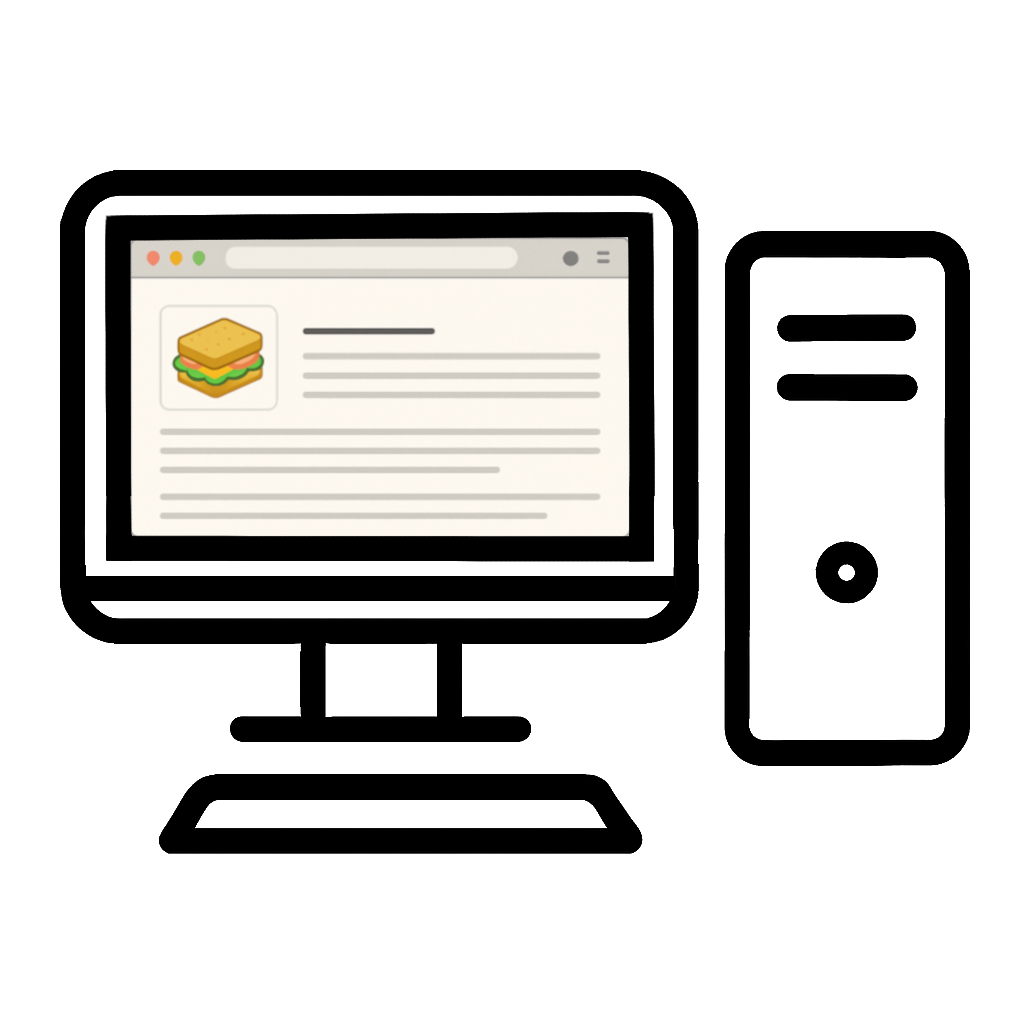
\includegraphics[width=1\textwidth]{./figures/computer_alpha_screen_2_website.png}
			\end{minipage}
		\end{adjustbox}
		\arrowx{\text{information}}
		\begin{adjustbox}{scale=1}
			\begin{minipage}{1\textwidth}
				
\includegraphics[width=0.8\textwidth]{./figures/evil_computer_scientist_alpha.png}
			\end{minipage}
		\end{adjustbox}
	\end{transformation}
	\vspace{-0.5cm}
	\begin{itemize}
		\item Information collected through web browser
		\item Privacy risk
	\end{itemize}
\end{frame}

\begin{frame}[fragile]{Introduction}{Browser-based device tracking}
	\begin{columns}
		\begin{column}{0.33\textwidth}
			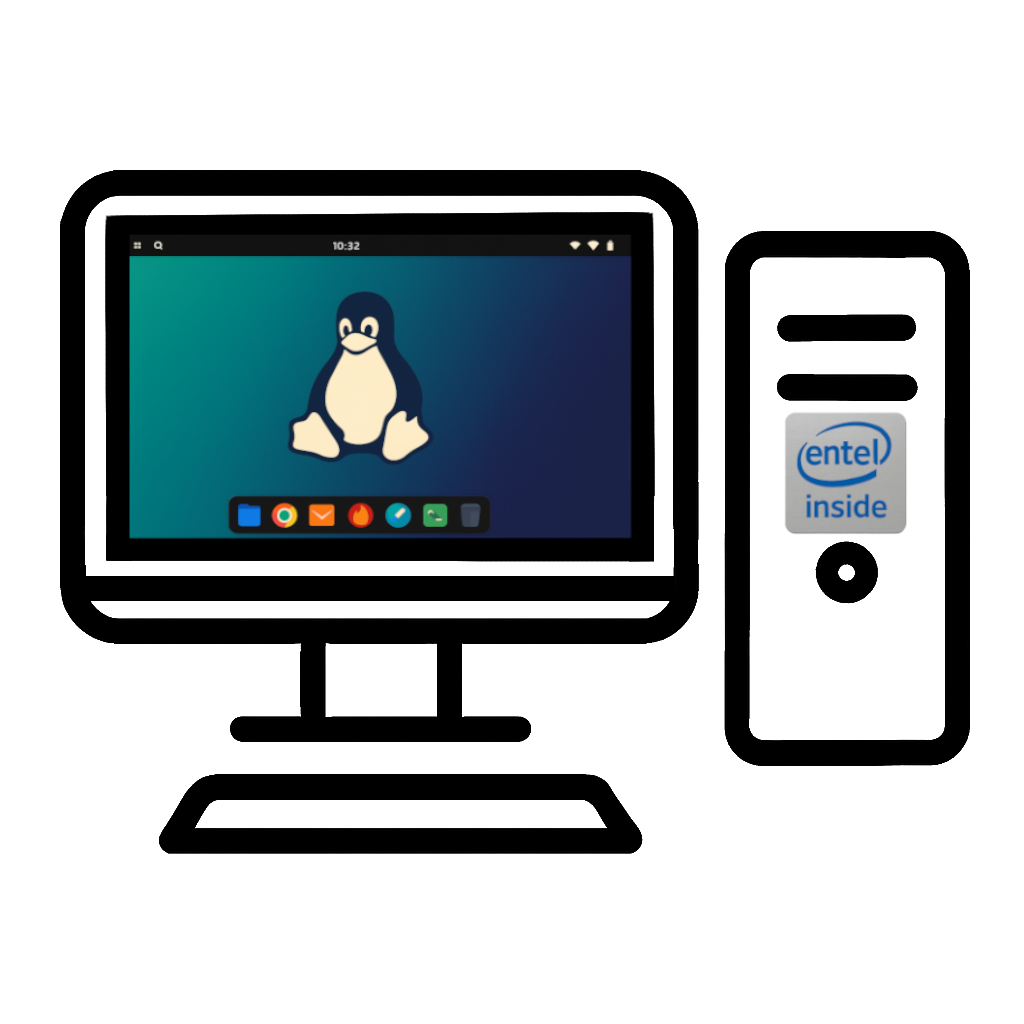
\includegraphics[width=1\textwidth]{./figures/computer_alpha_screen_2_golden.png}
		\end{column}
		\begin{column}{0.33\textwidth}
			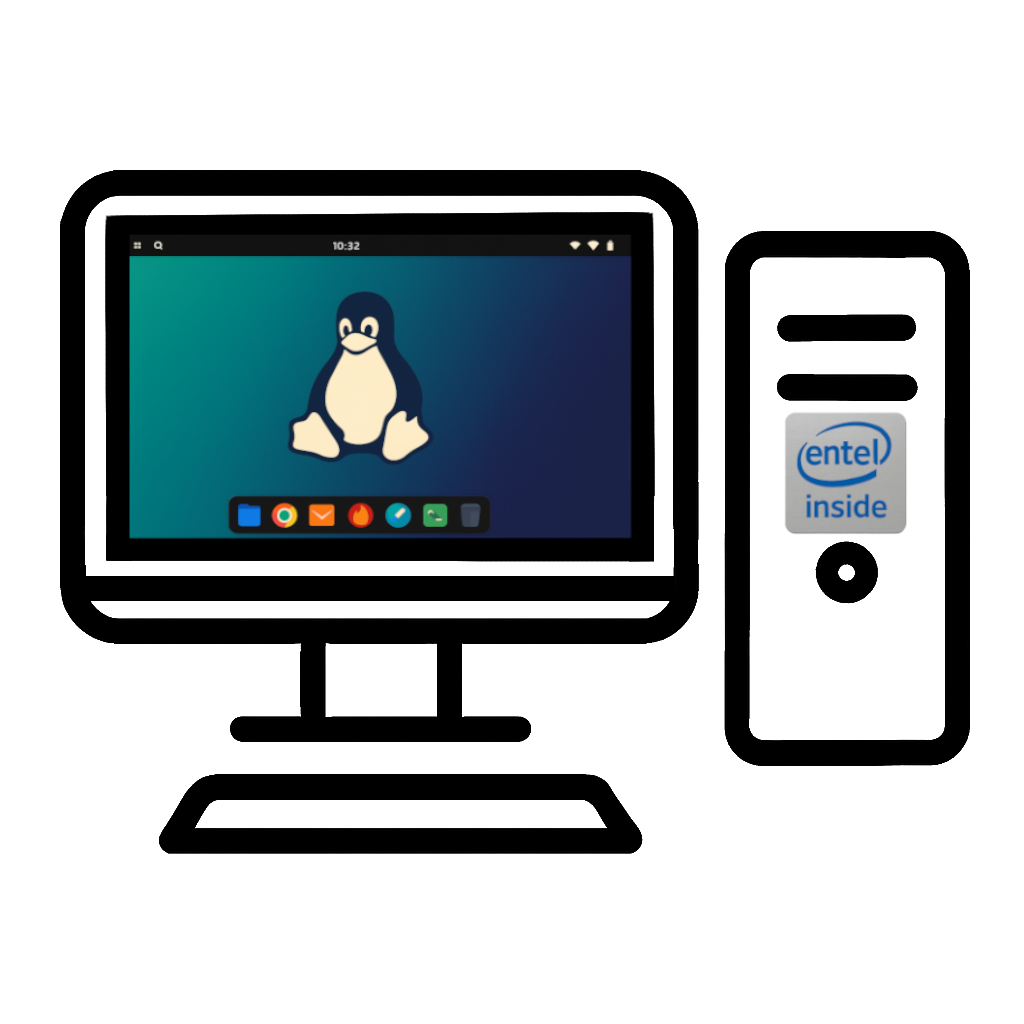
\includegraphics[width=1\textwidth]{./figures/computer_alpha_screen_2_golden.png}
		\end{column}
		\begin{column}{0.33\textwidth}
			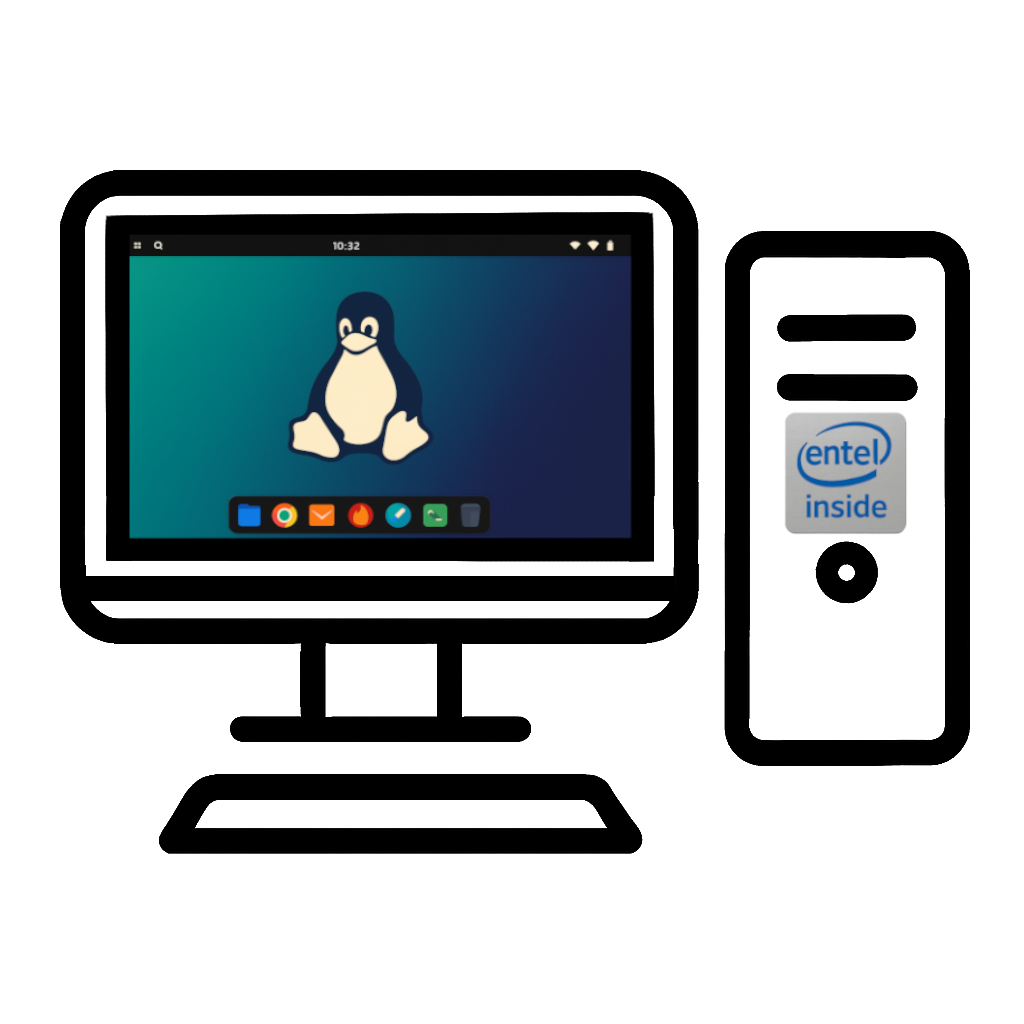
\includegraphics[width=1\textwidth]{./figures/computer_alpha_screen_2_golden.png}
		\end{column}
	\end{columns}
	\vspace{-0.5cm}
	\begin{itemize}
		\item \alert{Golden image challenge:} Distinguish identical devices with same hardware and software configuration \checkboxUnchecked \alert{$\Rightarrow$ device-specific key}
	\end{itemize}
\end{frame}

\begin{frame}[fragile]{Introduction}{Browser-based device tracking}
	\begin{itemize}
		\item \alert{Tagging techniques:} Insert an ID
		\begin{columns}
			\begin{column}{0.33\textwidth}
				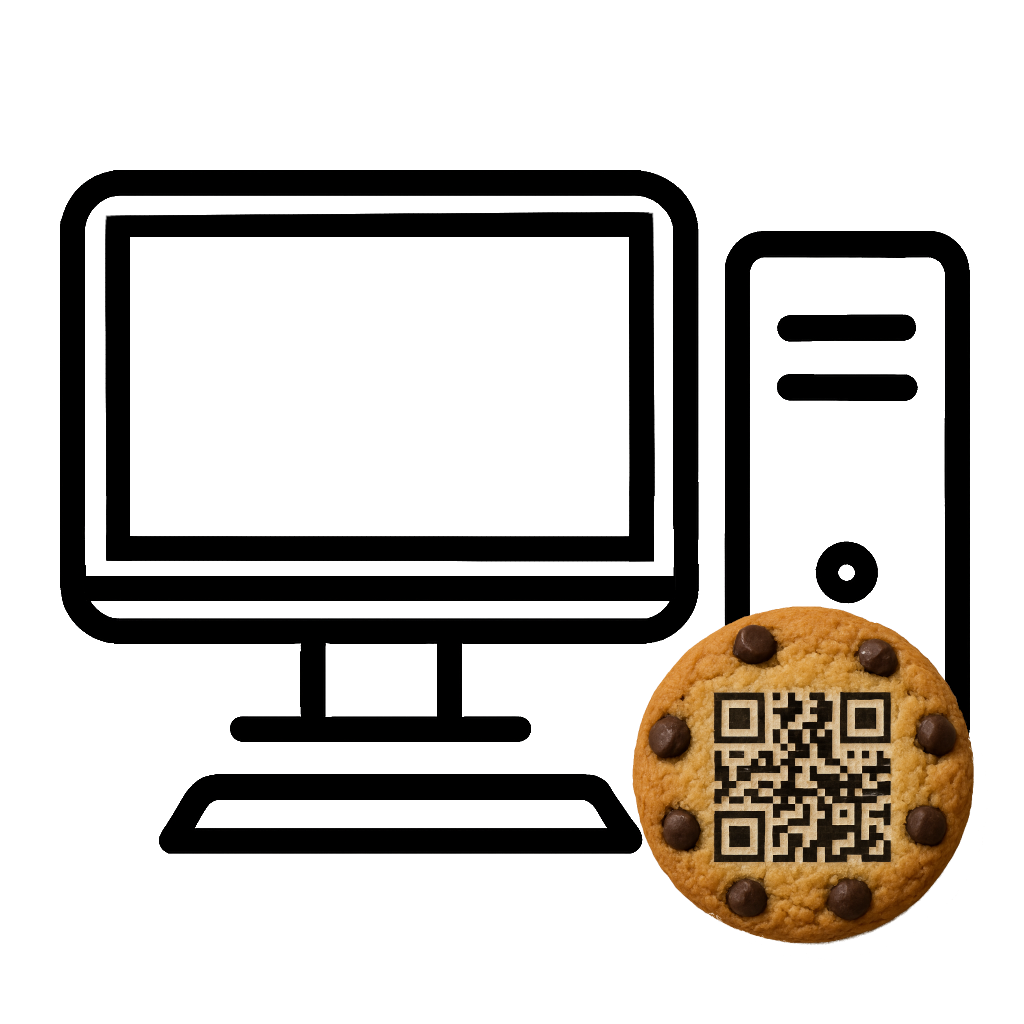
\includegraphics[width=0.5\textwidth, center]{./figures/computer_alpha_cookie_1.png}
			\end{column}
			\begin{column}{0.33\textwidth}
				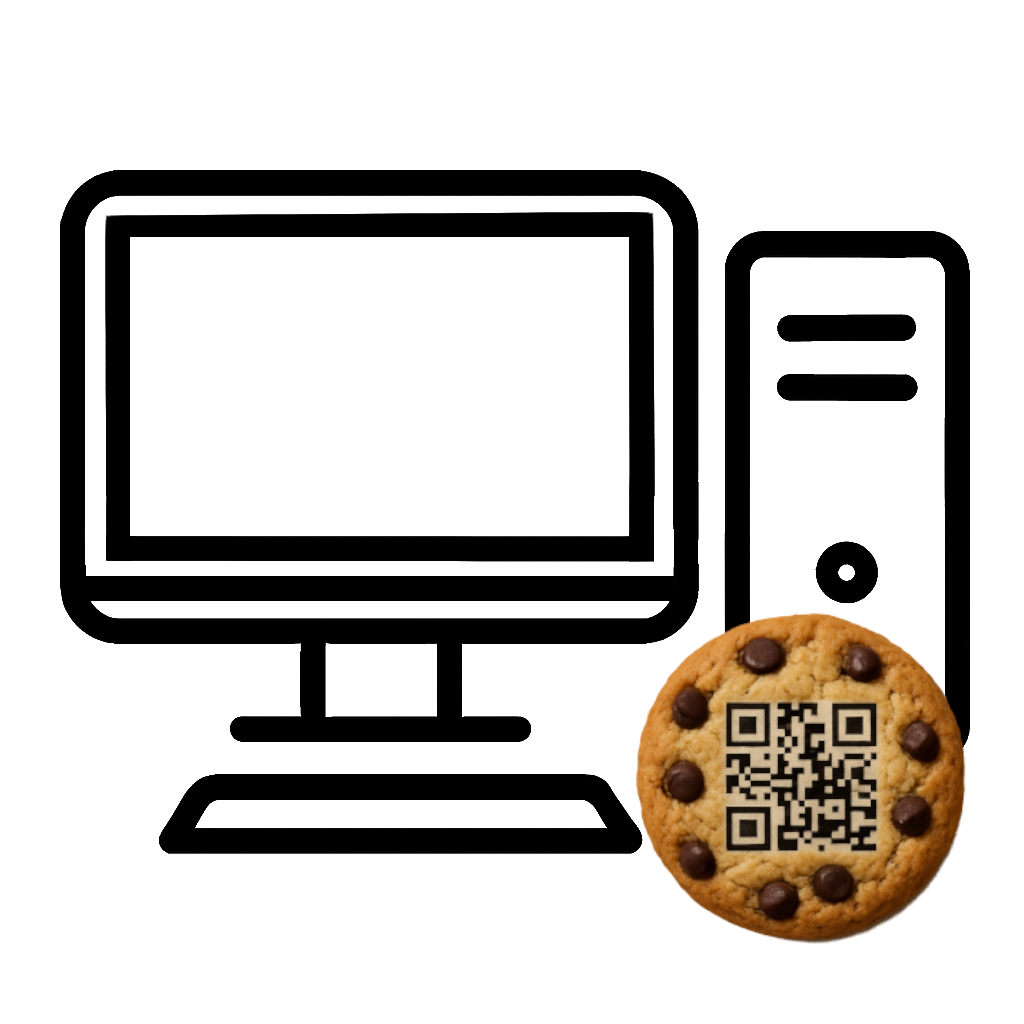
\includegraphics[width=0.5\textwidth, center]{./figures/computer_alpha_cookie_2.png}
			\end{column}
			\begin{column}{0.33\textwidth}
				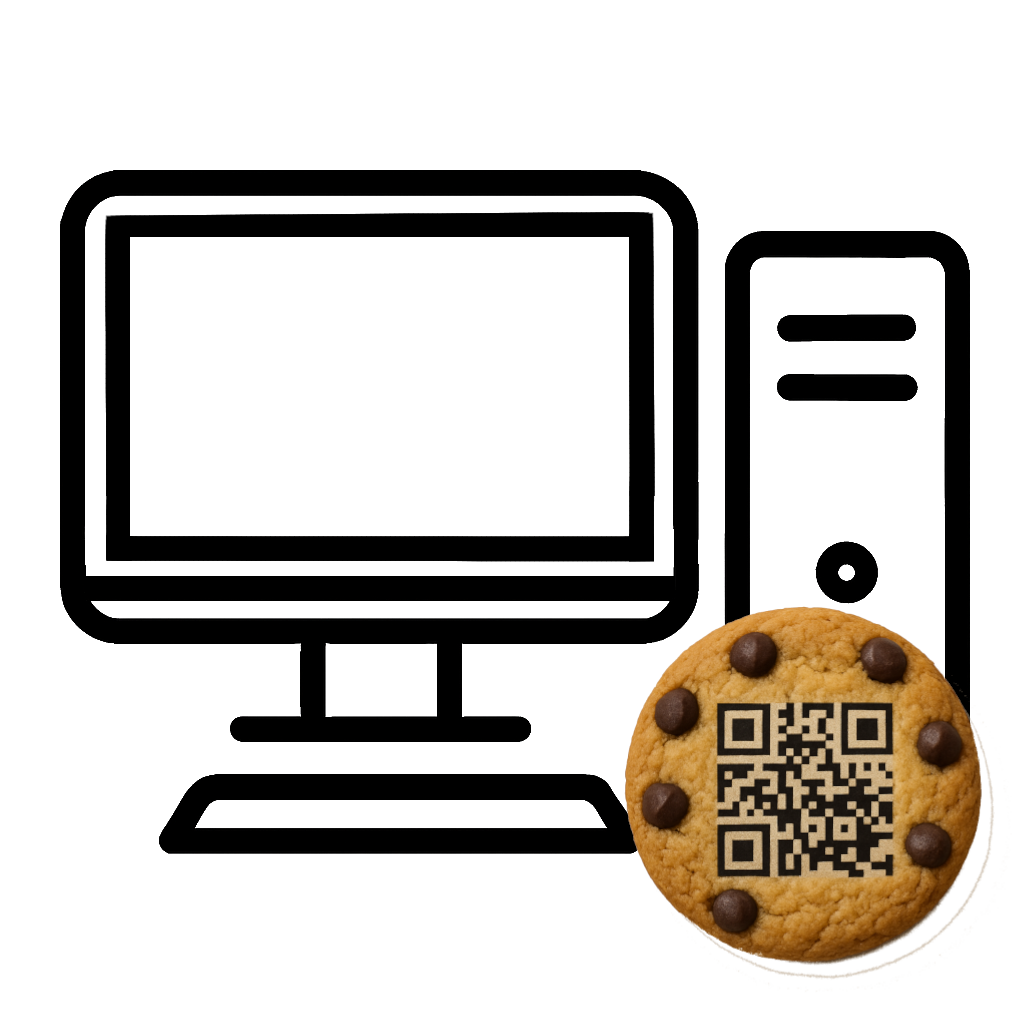
\includegraphics[width=0.5\textwidth, center]{./figures/computer_alpha_cookie_3.png}
			\end{column}
		\end{columns}
		\item \alert{Fingerprinting techniques:} Measure characteristics
		\begin{center}
			\begin{minipage}{0.7\textwidth}
				\begin{transformation}
					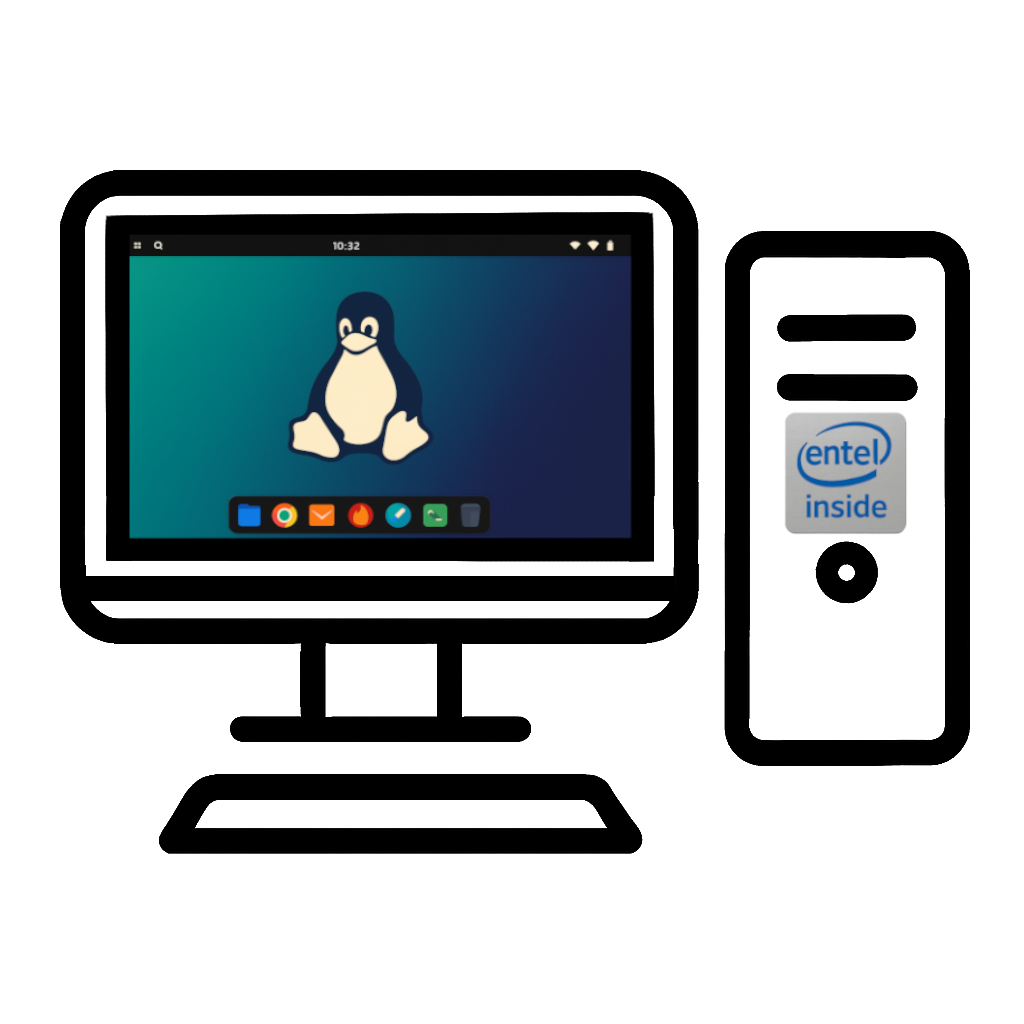
\includegraphics[width=0.7\textwidth]{./figures/computer_alpha_screen_2_golden.png}
					\arrowx{\text{generate fingerprint}}
					
\includegraphics[width=0.3\textwidth]{./figures/fingerprint.png}
				\end{transformation}
			\end{minipage}
		\end{center}
	\end{itemize}
	\begin{tikzpicture}[remember picture, overlay, shift={(current page.south west)}]
		\draw[thick, draw=PrimaryColor] (0.6cm,1.1cm) rectangle (13.2cm,4.2cm);
	\end{tikzpicture}
	% \grid
\end{frame}

\begin{frame}[fragile]{Introduction}{Source Port Selection}
	\begin{itemize}
		\item \alert{4-tuple}: $(IP_{Src}, Port_{Src}, IP_{Dest}, Port_{Dest})$
		\begin{transformation}[0.2][0.6][0.2]
			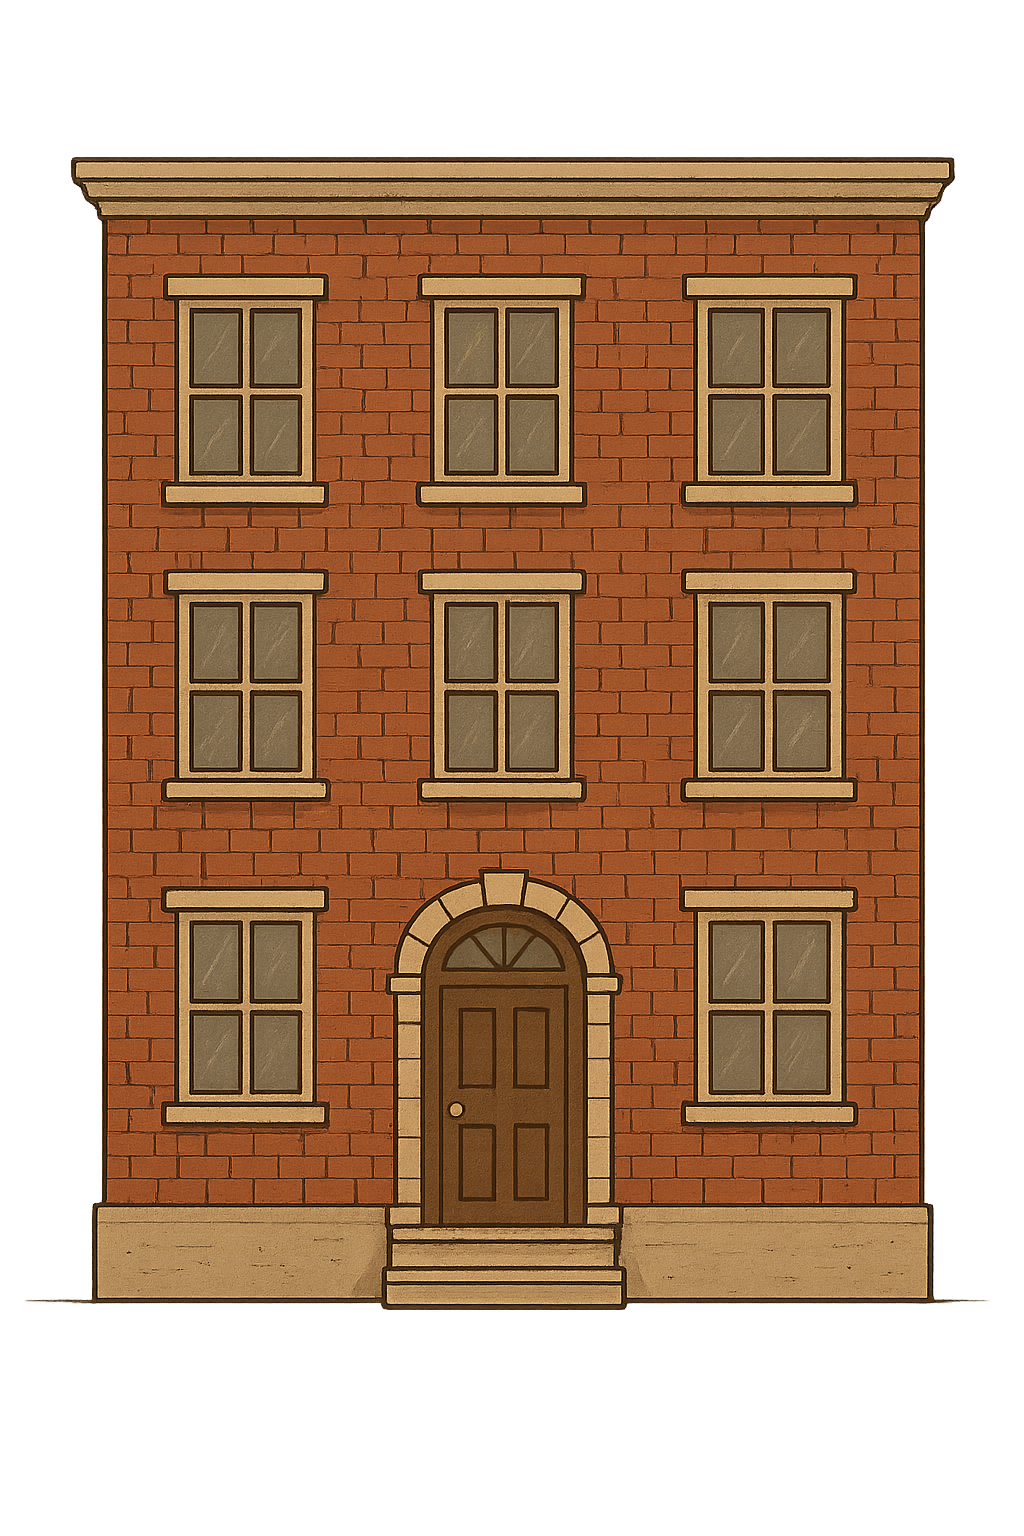
\includegraphics[width=\textwidth]{./figures/apartment1.png}
			\arrowxx{\text{(123 Maple St., Apt. 5B)}\hspace{1cm}\text{(456 Oak St., Apt. 9D)}}{\text{(10.0.0.12, 49210)}\hspace{1cm}\text{(74.125.133.109, 587)}}
			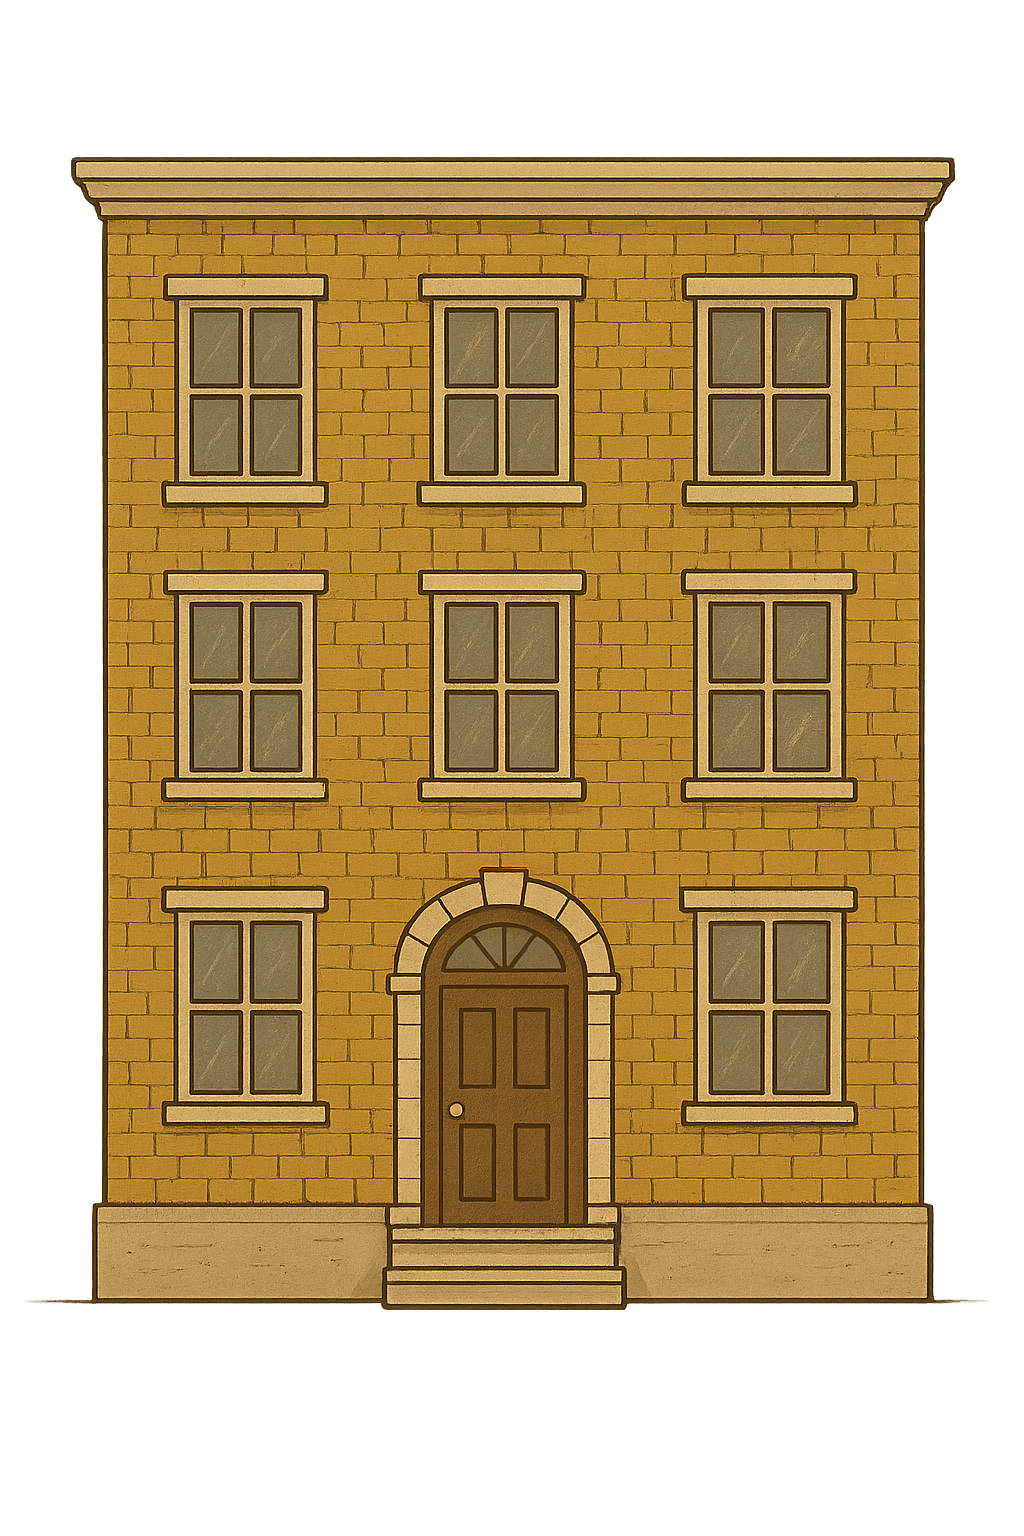
\includegraphics[width=\textwidth]{./figures/apartment2.png}
		\end{transformation}
		\vspace{-0.4cm}
		\begin{itemize}
			\scriptsize
			\item (10.0.0.12, 49210, 74.125.133.109, 587)
			\item (123 Maple St., Apt. 5B, 456 Oak St., Apt. 9D
		\end{itemize}
		\item Chooses TCP \alert{source port} $Port_{Src}$ for \alert{3-tuple}: $(IP_{Src}, IP_{Dest}, Port_{Dest})$
	\end{itemize}
\end{frame}

\begin{frame}[fragile]{Introduction}{Source Port Selection}
	\begin{itemize}
		\item \alert{Functionality:} Reusing soure ports can cause failures
		\begin{itemize}
			\item[\alert{$\Rightarrow$}] Earlier connections might be active (\texttt{TIME\_WAIT} state)
		\end{itemize}
	\end{itemize}
	\begin{columns}
		\begin{column}[t]{0.33\textwidth}
			\vspace{2cm}

			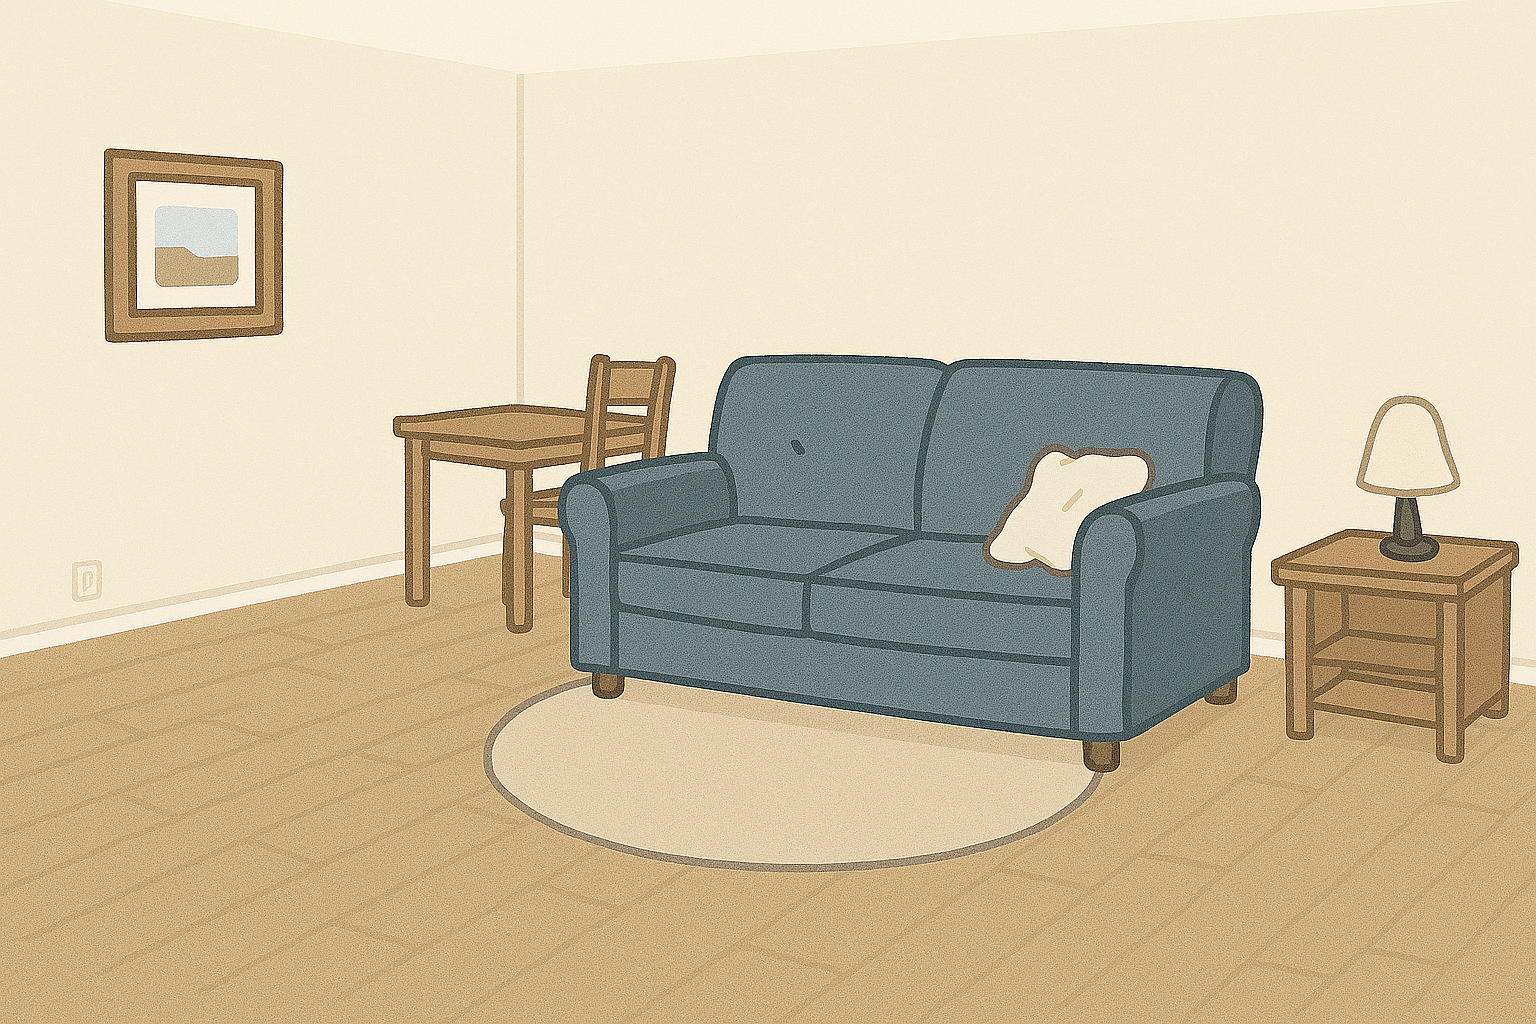
\includegraphics[width=0.8\textwidth, center]{./figures/room_cleaned.png}
		\end{column}
		\begin{column}[t]{0.33\textwidth}
			\vspace{0cm}

			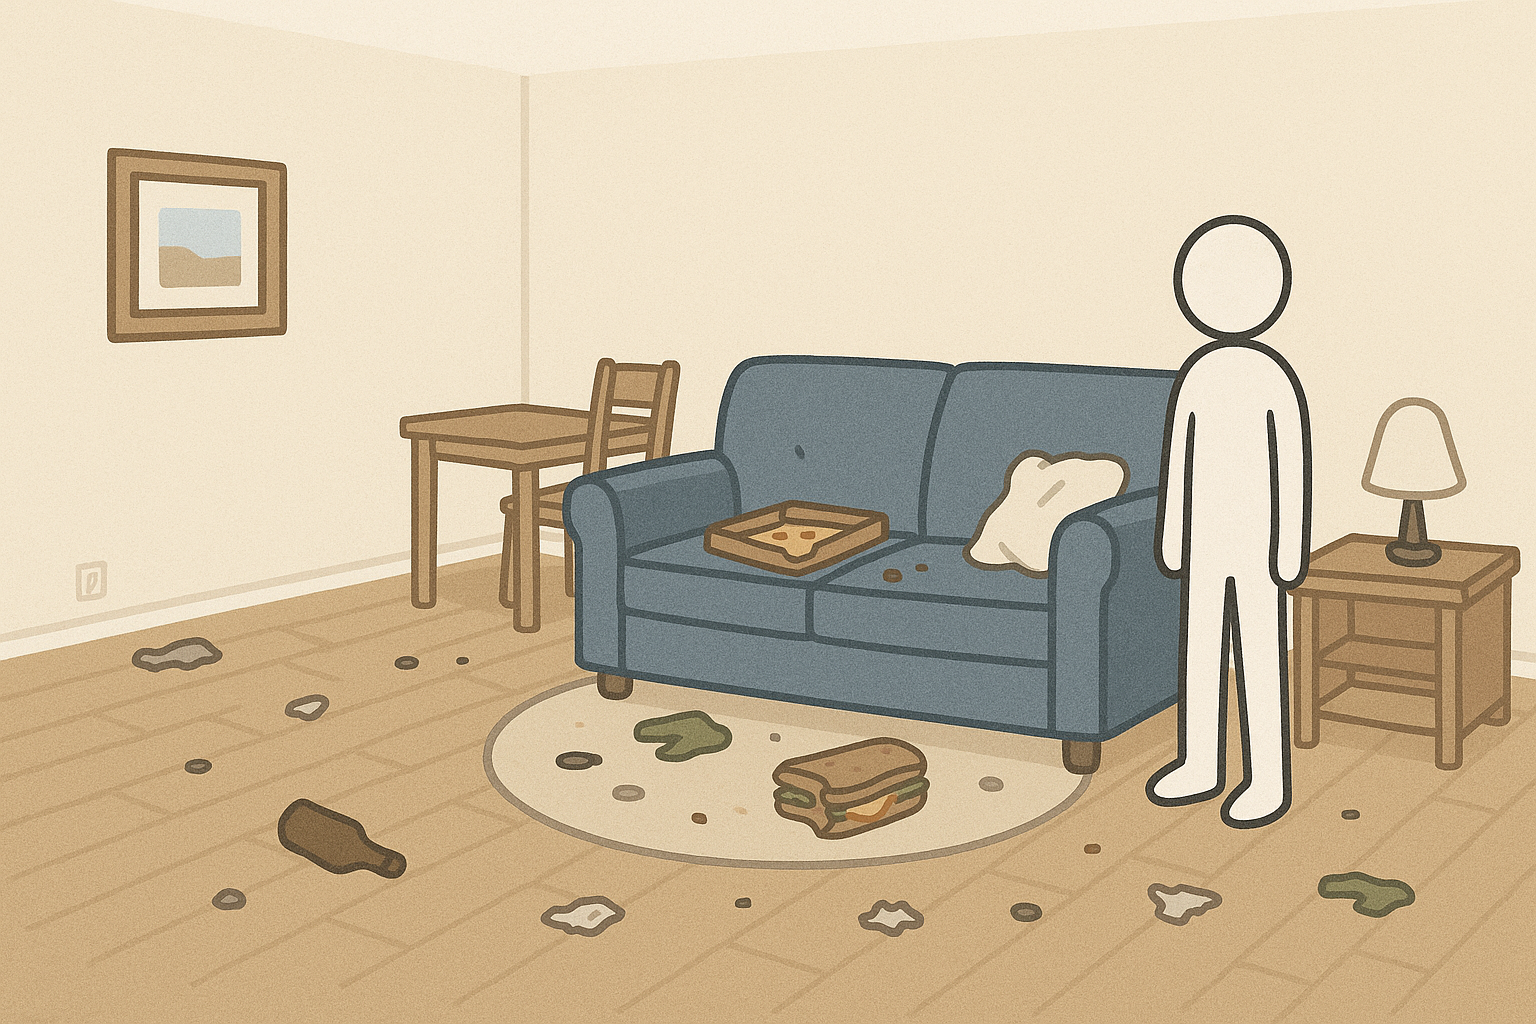
\includegraphics[width=0.8\textwidth, center]{./figures/room_not_cleaned.png}
		\end{column}
		\begin{column}[t]{0.33\textwidth}
			\vspace{0cm}

			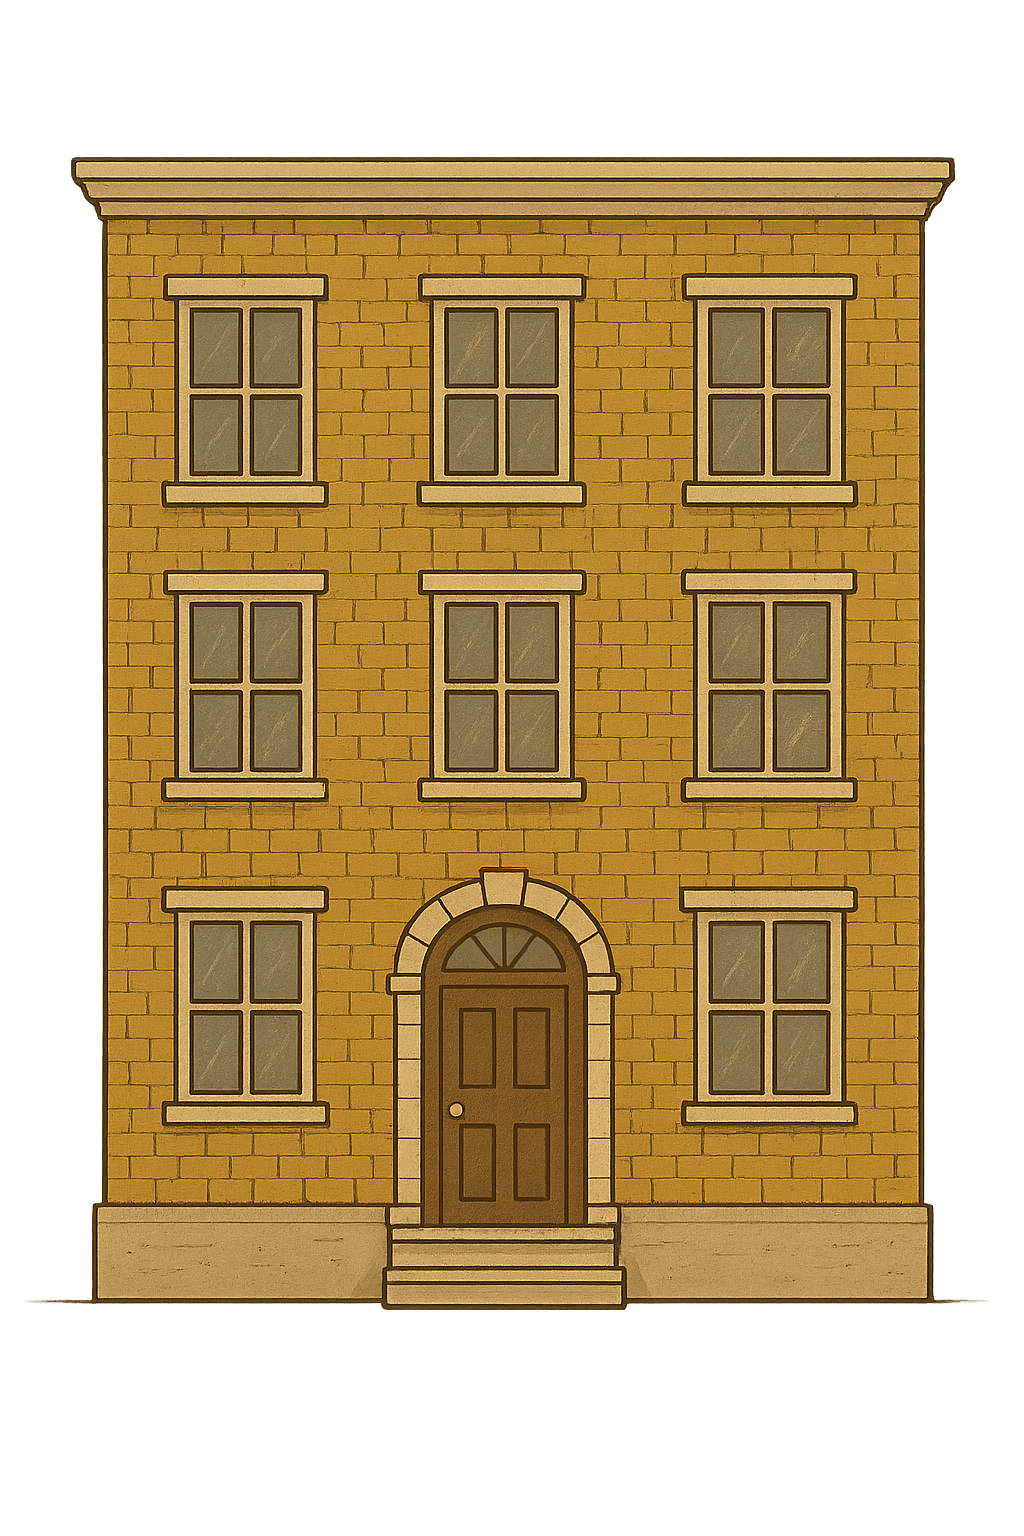
\includegraphics[width=0.8\textwidth, center]{./figures/apartment2.png}
		\end{column}
	\end{columns}
	\begin{tikzpicture}[remember picture, overlay, shift={(current page.south west)}]
		\draw[->, thick, draw=PrimaryColor] (4.35,2.3) -- (10.8,1.95);
		\draw[->, thick, draw=PrimaryColor] (9.1,4.3) -- (11.7,3.1);
	\end{tikzpicture}
	% \grid
\end{frame}

\begin{frame}[fragile]{Introduction}{Source Port Selection}
	\begin{itemize}
		\item \alert{Security:}
		\begin{itemize}
			\item \alert{Off-path attacks} %like blind reset, data injection
			\item Determine \alert{Device activity (number TCP connections per time)} % if an attacker could, e.g., force a client to periodically establish a new TCP connection to an attacker-controlled machine (or through an attacker- observable path), the attacker could subtract consecutive source port values to obtain the number of outgoing TCP connections established globally by the target host within that time period 
		\end{itemize}
		\begin{transformation}[0.2][0.6][0.2]
			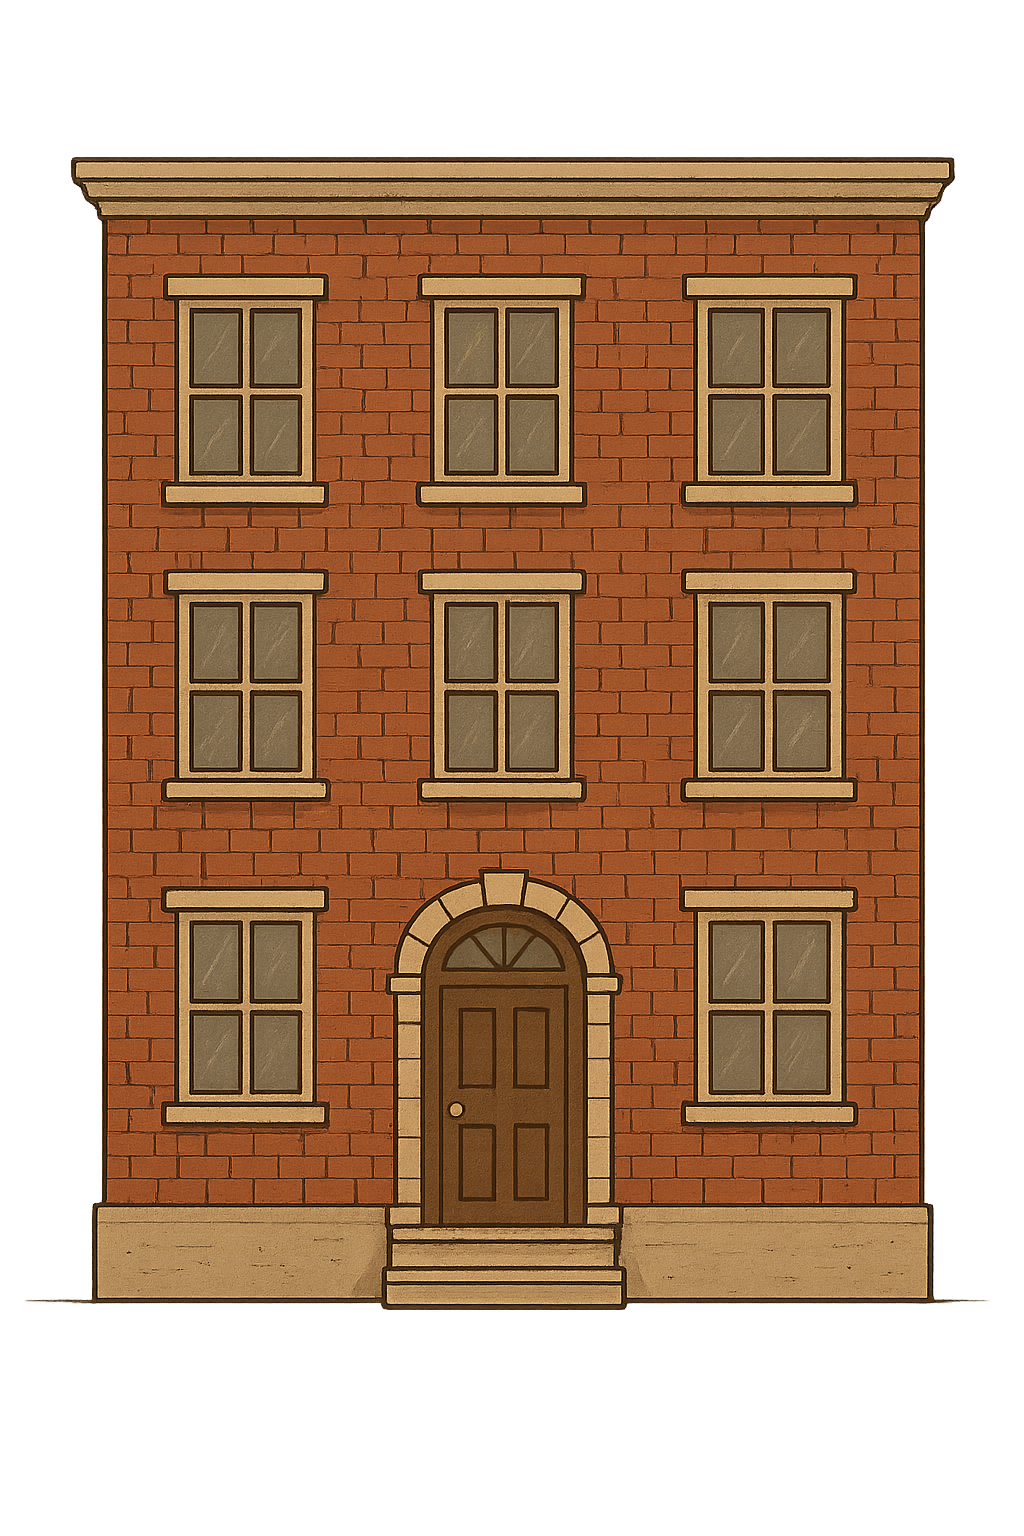
\includegraphics[width=\textwidth]{./figures/apartment1.png}
			\arrowxx{
\includegraphics[width=0.3\textwidth]{./figures/evil_computer_scientist_bicycle.png}}{\text{(123 Maple St., Apt. 5B)}\hspace{1cm}\text{(456 Oak St., Apt. 9D)}}
			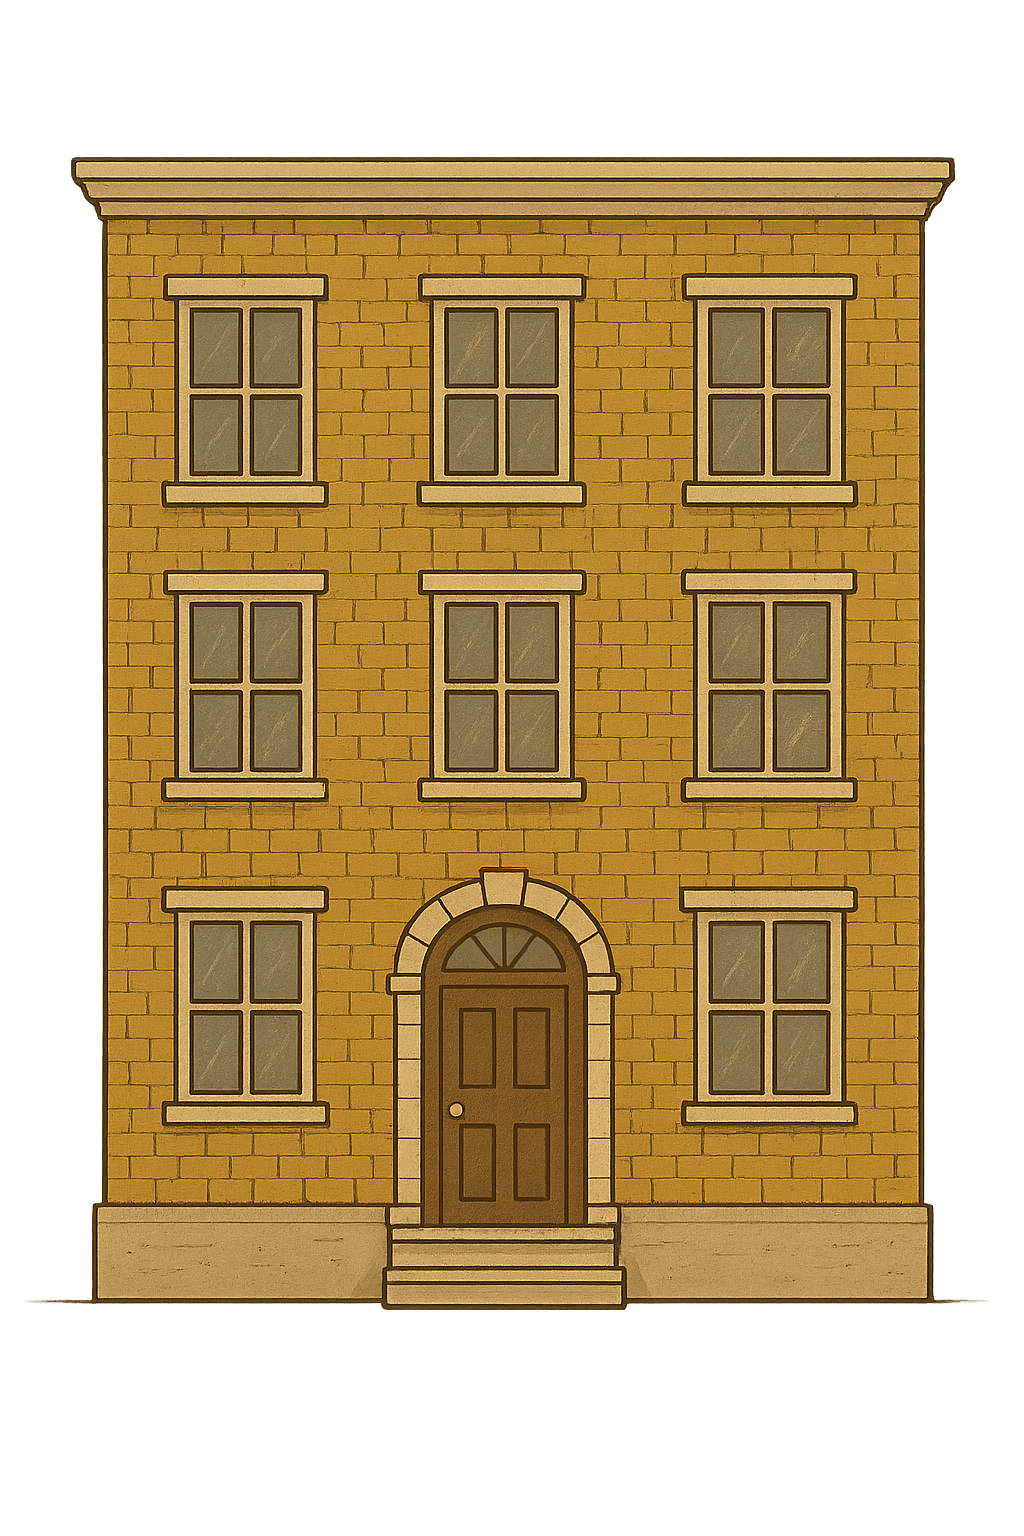
\includegraphics[width=\textwidth]{./figures/apartment2.png}
		\end{transformation}
	\end{itemize}
\end{frame}

\begin{frame}[fragile]{Introduction}{Double-Hash Port Selection Algorithm (DHPS)}
	\begin{itemize}
		\item TCP source ports divided into \alert{ranges}:

		\begin{adjustbox}{max width=0.9\textwidth}
			\begin{tblr}{
				colspec={|l|c|p{7cm}|},
				hlines,
				vlines,
				colsep=5pt,
				row{1} = {bg=PrimaryColor, fg=white, font=\bfseries},
				row{2} = {bg=PrimaryColorDimmed},
				row{3} = {bg=SecondaryColorDimmed},
				row{4} = {bg=PrimaryColorDimmed}
				}
				Port Range Type  & Typical Range & Usage                                                               \\
				Well-known ports & 0–1023        & Specific services, e.g. HTTP (80), HTTPS (443) etc.                 \\
				Registered ports & 1024–49151    & User applications or services, not ephemeral                        \\
				Ephemeral ports  & 49152–60999   & Dynamically allocated by OS for short-lived client-side connections \\
			\end{tblr}
		\end{adjustbox}
	\end{itemize}
	\begin{tikzpicture}[remember picture, overlay, shift={(current page.south west)}]
		\draw[thick, draw=PrimaryColor] (1.15cm,2.23cm) rectangle (13.5cm,3.22cm);
		\draw[->, thick, draw=PrimaryColor] (14.4,2.75) -- (13.6,2.75);
	\end{tikzpicture}
	% \grid
\end{frame}

\begin{frame}[fragile]{Introduction}{Double-Hash Port Selection Algorithm (DHPS)}
	\begin{itemize}
		\item \alert{Complete 3-tuple to 4-tuple} with cryptographic keyed-hash functions:
		\begin{itemize}
			\scriptsize
			\item \( F_{K_1}: \text{3-Tuples} \xrightarrow{K_1} \{0, \ldots, 2^{32}\}\)
			\item \( G_{K_2}: \text{3-Tuples} \xrightarrow{K_2} \{0, \ldots, T\}\) where $T$ is length of \alert{perturbation table}
		\end{itemize}
	\end{itemize}
	\begin{columns}
		\begin{column}{0.5\textwidth}
			\begin{itemize}
				\item Incrementation of port numbers separated into \alert{$T$ different spaces}
				\begin{itemize}
					\item[\alert{$\Rightarrow$}] Port-reuse frequency lower % (probabilistically) 
					\item[\alert{$\Rightarrow$}] Harder to analyse device activity % if an attacker could, e.g., force a client to periodically establish a new TCP connection to an attacker-controlled machine (or through an attacker- observable path), the attacker could subtract consecutive source port values to obtain the number of outgoing TCP connections established globally by the target host within that time period
				\end{itemize}
			\end{itemize}
		\end{column}
		\begin{column}{0.5\textwidth}
			\begin{center}
				\begin{adjustbox}{max width=\textwidth}
					\tikzfig{perturbation_table}
				\end{adjustbox}
			\end{center}
		\end{column}
	\end{columns}
	% Further increasing the TABLE_LENGTH will increase the unpredictability of the resulting port number, and possibly further decrease the collision rate
\end{frame}

\begin{frame}[fragile]{Introduction}{Double-Hash Port Selection Algorithm (DHPS)}
	\begin{adjustbox}{scale=0.8}
		\begin{minipage}{0.8\textwidth}
			%!Tex Root = ../main.tex

\begin{algorithm}{\pr{DHPS Source Port Selection}}{\thetcbcounter}\label{alg:dhps_port_selection}
	\begin{pseudo}[indent-mark,kw,hl-warn=false]
		procedure \cn{SelectEphemeralPort} \\+
		\tt{num\_ephemeral} $\leftarrow \tt{max\_ephemeral} - \tt{min\_ephemeral}+\tn{1}$ \\
    \tt{offset} $\leftarrow$ $\cn{F}_{K_1}$($\tt{IP}_{SRC}$,$\tt{IP}_{DST}$,$\tt{PORT}_{DST}$) \\
    \tt{index} $\leftarrow$ $\cn{G}_{K_2}$($\tt{IP}_{SRC}$,$\tt{IP}_{DST}$,$\tt{PORT}_{DST}$) \\
		\tt{count} $\leftarrow$ \tt{num\_ephemeral} \\
		repeat \\+
		$\tt{port} $\leftarrow$ \tt{min\_ephemeral}$+\\+
		$((\tt{offset}+\tt{table[index]})$ $mod$ $\tt{num\_ephemeral})$ \\-
		$\tt{table[index]} $\leftarrow$ \tt{table[index]} +\tn{1}$ \\
		if \cn{CheckSuitablePort}(\tt{port}) then \\+
		return \tt{port} \\-
		$\tt{count} $\leftarrow$ \tt{count} - \tn{1}$ \\-
		until \tt{count} = \tn{0} \\
		return \tt{Error}\\
	\end{pseudo}
\end{algorithm}

		\end{minipage}
	\end{adjustbox}
	% \begin{tikzpicture}[remember picture, overlay, shift={(current page.south west)}] % 1
	% 	\node[anchor=north west]  at (9.3cm, 5.8cm) {%
	% 		\includegraphics[scale=0.7]{./figures/external/dhps_source_port_calculation_2.pdf}
	% 	};
	% \end{tikzpicture}
	% \begin{tikzpicture}[remember picture, overlay, shift={(current page.south west)}]
	% 	\node[anchor=north west] at (9cm, 7.1cm) {%
	% 		\begin{minipage}{\textwidth}
	% 			\begin{itemize}
	%          \item \alert{Source port calculation:}
	% 				\begin{itemize}
	%            \scriptsize
	% 					\item $offset=50'000$
	% 					\item $index=255$
	% 				\end{itemize}
	% 			\end{itemize}
	% 		\end{minipage}
	% 	};
	% \end{tikzpicture}
	\begin{tikzpicture}[remember picture, overlay, shift={(current page.south west)}] % 2
		\node[anchor=north west]  at (9.3cm, 5.8cm) {%
			\includegraphics[scale=0.7]{./figures/external/dhps_source_port_calculation_increment.pdf}
		};
	\end{tikzpicture}
	\begin{tikzpicture}[remember picture, overlay, shift={(current page.south west)}]
		\node[anchor=north west] at (9cm, 7.1cm) {%
			\begin{minipage}{\textwidth}
				\begin{itemize}
					\item \alert{Source port calculation:}
					\begin{itemize}
						\scriptsize
						\item $offset=50'000$
						\item $index=255$
					\end{itemize}
				\end{itemize}
			\end{minipage}
		};
	\end{tikzpicture}
	\begin{tikzpicture}[remember picture, overlay, shift={(current page.south west)}]
		% source port calculation % 1
		% \draw[thick, draw=PrimaryColor] (1.55cm,5.0cm) rectangle (6.85cm,5.45cm);
		% \draw[thick, draw=PrimaryColor] (1.55cm,4.6cm) rectangle (6.75cm,5.0cm);
		% \draw[thick, draw=PrimaryColor] (2.15cm,3.1cm) rectangle (9.25cm,3.9cm);
		% increase of table entry % 2
		\draw[thick, draw=PrimaryColor] (2.15cm,2.75cm) rectangle (6.95cm,3.1cm);
		\draw[thick, draw=PrimaryColor] (2.15cm,1.95cm) rectangle (7.35cm,2.75cm);
		% loop termiation
		% \draw[thick, draw=PrimaryColor] (1.55cm,4.25cm) rectangle (4.9cm,4.6cm);
		% \draw[thick, draw=PrimaryColor] (2.15cm,1.6cm) rectangle (4.65cm,1.95cm);
		% \draw[thick, draw=PrimaryColor] (1.55cm,1.2cm) rectangle (3.85cm,1.6cm);
		% terminate with error
		% \draw[thick, draw=PrimaryColor] (1.55cm,0.75cm) rectangle (3.45cm,1.2cm);
	\end{tikzpicture}
	% \grid
\end{frame}

\section{Attack}

\begin{frame}[fragile]{Attack}{Parties}
	\centering
	\begin{adjustbox}{max width=\textwidth}
		\tikzfig{sequence_diagram_attack} % ./figures/sequence_diagram_attack.tikz
	\end{adjustbox}
\end{frame}

\begin{frame}[fragile]{Attack}{Phase 1}
	\begin{center}
		\begin{adjustbox}{scale=0.7}
			%!Tex Root = ../main.tex

\begin{algorithm}{\pr{Finding Attacker 3-Tuple per Cell (Phase 1)}}{\thetcbcounter}
	\begin{pseudo}[indent-mark,kw,hl-warn=false]
    procedure \cn{SendBurst}(\tt{X})\\+
    for all \tt{x} $\in$ \tt{X} do\\+
\cn{AttemptConnectTCP}(\tt{x})\\--
procedure \cn{GetSourcePorts}(\tt{U})\\+
\cn{SendBurst}(\tt{U})\\
\tt{R} $\leftarrow$ \cn{ReceiveAttackerTupleToPortMap}()\\
\cmt{// R = $\{(\tt{IP}_{SRC}$,$\tt{IP}_{DST}$,$\tt{PORT}_{DST}$) $\mapsto \tt{PORT}_{SRC}\}$}\\
\cmt{// (obtained from the tracking server)}\\
return \tt{R}\\-
procedure \cn{Phase1}\\+
\tt{S'} $\leftarrow\emptyset$\\
while $|\tt{S'}| < \tt{T}$ do\\+
$\tt{S}_i$ $\leftarrow$ \cn{GetNewExternalDestinations}()\\
\cmt{// $\forall_{j<i}(\tt{S}_i \cap \tt{S}_j = \emptyset)$}\\
\tt{P} $\leftarrow$ \cn{GetSroucePorts}($\tt{S}_i$) \cmt{// 1st burst}\\
\cn{SendBurst}(S') \cmt{// 2nd burst}\\
\tt{P'} $\leftarrow$ \cn{GetSourcePorts}($\tt{S}_i$) \cmt{// 3rd burst}\\
\tt{S'} $\leftarrow \tt{S'} \cup \{x\,|\,\tt{P'}(x)−\tt{P}(x)=1\}$\\
\cmt{// $\tt{V}_i = \{\tt{x}\,|\,\tt{P'}(x)-\tt{P}(x) = 1\}$}\\-
return \tt{S'}
	\end{pseudo}
\end{algorithm}

		\end{adjustbox}
	\end{center}
\end{frame}

\begin{frame}[fragile]{Attack}{Phase 2}
	\begin{center}
		\begin{adjustbox}{scale=0.7}
			%!Tex Root = ../main.tex

\begin{algorithm}{\pr{Finding a Device ID (Phase 2)}}{\thetcbcounter}\label{alg:phase2}
	\begin{pseudo}[indent-mark,kw,hl-warn=false]
procedure \cn{Phase2}\\+
$\tt{C} \leftarrow \emptyset; \tt{n} \leftarrow 0; \tt{i} \leftarrow 0$\\
repeat\\+
$\tt{i} \leftarrow \tt{i}+1$\\
$\tt{C} \leftarrow \cn{GetSourcePorts}(\tt{S'})$ \cmt{// 1st burst}\\
\cn{AttemptConnectTCP}\tn{(}$\{\tt{L}_i\}$\tn{)} \cmt{// 2nd burst}\\
$\tt{C'} \leftarrow \cn{GetSourcePorts}\tn{(}\tt{S'})$ \cmt{// 3rd burst}\\
$\tt{w} \leftarrow \text{\iota}w(\tt{C'}(w) - \tt{C}(w) > \tn{\varepsilon})$\\
if \cn{Defined}\tn{(}$\tt{B}_w$\tn{)} then \cmt{// A collision was found}\\+
$\tt{p} \leftarrow p \cup \{(\tt{L}_i,\tt{B}[w])\}$\\
$\tt{n} \leftarrow n+1$\\-
else\\+
$\tt{B}[w] \leftarrow L_i$\\--
until $\tt{n} \ge \tt{n}^*[i]$ \cmt{// This is equiv. to $P^N_T(i, n) \le p^*$}\\
return \tn{(}\tt{p},\tt{i}\tn{)}\\-
	\end{pseudo}
\end{algorithm}

		\end{adjustbox}
	\end{center}
\end{frame}

\section{Countermeasures}

\begin{frame}[fragile]{Countermeasures}{Possible solutions}
\end{frame}

\section{Appendix Work}

\begin{frame}[fragile]{Appendix}{Related Work}
\end{frame}

\begin{frame}[fragile]{Appendix}{Termination condition for phase 2}
\end{frame}

\section{Literature}

\begin{frame}[allowframebreaks]{Literature}
	% print publications
	% \printbibliography[category=myarticles,heading=subbibliography]
	\printbibliography
\end{frame}
%
% \begin{frame}[allowframebreaks]{Websites}
% 	\printbibliography[type=online,heading=subbibliography]
% \end{frame}
%
% \begin{frame}[allowframebreaks]{Images}
% 	\printbibliography[type=artwork,heading=subbibliography]
% 	\printbibliography[category=myimages,heading=subbibliography]
% \end{frame}

% \begin{frame}[allowframebreaks]{Literature} % {Online}
%   \nocite{palswimAnswerCreateCustom2019}\nocite{tinoAnswerHowGet2020}\nocite{CallingTextMateOther}
%   % \printbibliography[type=online,heading=subbibliography,title={Online}]
%   \printbibliography[heading=none]
% \end{frame}

% \begin{frame}{Sonstiges}
%   \printbibliography[nottype=book, nottype=article, nottype=online, nottype=unpublished,heading=subbibliography,title={Sonstige Quellen}]
% \end{frame}
\end{document}
